\documentclass[9pt,twoside]{extarticle}
\usepackage[T1]{polski}
\usepackage[utf8]{inputenc}
\usepackage{xcolor}
\usepackage{geometry}
%\usepackage[text=WERSJA\\ROBOCZA,fontsize=0.15\paperwidth,colorspec=0.95]{draftwatermark}
\usepackage{fontspec}
\usepackage{fancyhdr}
\usepackage{graphicx}
\usepackage[titles]{tocloft}
\usepackage{titlesec}


\geometry{
a6paper,
inner=19mm,
outer=10mm,
top=15mm,
bottom=15mm,
 }


\usepackage[
  width=11.1truecm, height=15.4truecm,
  cam, noaxes, frame, cross, pdftex, center, noinfo
%    noaxes, pdftex, center, noinfo
]{crop}


%\definecolor{RCRED}{RGB}{135, 24, 1}
\definecolor{RCRED}{RGB}{145, 8, 3}
\setmainfont{HelveticaNeue}
\newfontfamily{\trr}[Color=RCRED]{Times New Roman}
\newfontfamily{\hnlr}[UprightFont={*-Light},Color=RCRED]{HelveticaNeue}
\newfontfamily{\hnlb}[UprightFont={*-Light}]{HelveticaNeue}
\newfontfamily{\hnb}[Color=000000]{HelveticaNeue}
\newfontfamily{\hnr}[Color=RCRED]{HelveticaNeue}


\renewcommand{\baselinestretch}{1.15}


\newcommand{\ltrhdr}[1]{{\par\noindent\bf #1\par}}
\renewcommand{\headrulewidth}{0pt}


\newcommand{\gs}[1]{
  \cleardoublepage\section*{#1}
  \addcontentsline{toc}{section}{#1}
  \fancyhead[LE]{\hnb\tiny #1}
  \fancyhead[RO]{}
}


\newcommand{\gss}[1]{
  \subsection*{#1}
  \addcontentsline{toc}{subsection}{#1}
  \fancyhead[RO]{\hnb\tiny #1}
}


\newcommand{\gsss}[1]{
  \subsubsection*{#1}
  \addcontentsline{toc}{subsubsection}{#1}
}


\titleformat{\section}
  {\normalfont\fontsize{13}{16}\bfseries}{\thesection}{1em}{}


\titleformat{\subsection}
  {\normalfont\fontsize{11}{14}\bfseries}{\thesection}{1em}{}


\titleformat{\subsubsection}
  {\normalfont\fontsize{9}{12}\bfseries}{\thesection}{1em}{}


\titlespacing\section{0pt}{12pt plus 4pt minus 2pt}{0pt plus 2pt minus 2pt}
\titlespacing\subsection{0pt}{12pt plus 4pt minus 2pt}{0pt plus 2pt minus 2pt}
\titlespacing\subsubsection{0pt}{12pt plus 4pt minus 2pt}{0pt plus 2pt minus 2pt}




\begin{document}
%\sloppy
\pagestyle{fancy}


\begin{titlepage}
\setlength{\parindent}{0pt}
\vspace*{5cm}
\begin{flushright}
%\renewcommand{\arraystretch}{1.3}
\begin{tabular}{l@{}}
%{\Large Panie, ucz nas}\\
%{\hnlr\Huge MODLITWY}\\
{\fontsize{18pt}{36pt}\selectfont Panie, ucz nas}\\
\\
{\hnlr\fontsize{28pt}{42pt}\selectfont MODLITWY}\\
\\
\\
{\fontsize{14pt}{36pt}\selectfont Modlitewnik świeckich}\\
{\fontsize{14pt}{36pt}\selectfont członków Regnum Christi}
\\
\\
{\fontsize{10pt}{36pt}\selectfont Wydanie drugie poprawione}
\end{tabular}
\end{flushright}
\end{titlepage}


\setmainfont{Times New Roman}


\ \thispagestyle{empty}
\newpage




\fancyhf{}
\fancyfoot[LE]{\hnlb\tiny \strong{\thepage}{} | Regnum Christi}
\fancyfoot[RO]{\hnlb\tiny Legioniści Chrystusa \textbullet{} Kobiety konsekrowane \textbullet{} Mężczyźni konsekrowani \textbullet{} Świeccy | \strong{\thepage}}




\begin{center}




Przyjdź Królestwo Twoje!


\vspace{12pt}
{\trr REGNUM CHRISTI\\
\textcolor{RCRED}{\rule[4pt]{3cm}{0.4pt}}


{\tiny DYREKCJA GENERALNA\\
Via Aurelia 677 - 00165 Rzym, Włochy\par}}


\end{center}


\vspace{18pt}\par\noindent
Rzym, 16 grudnia 2022 r.


\vspace{6pt}\par\noindent
Do wszystkich członków Regnum Christi


\vspace{6pt}\par\noindent
Drodzy w Chrystusie


\vspace{6pt}
W trakcie Adwentu przygotowujemy nasz dom na przybycie wyjątkowego gościa: naszego Króla, który chce obudzić w nas pragnienie gościnności, przedstawiając się jako nowonarodzone Dziecię. Jest to czas porządkowania naszych domów i serc, czas oczekiwania i radości. To czas wspominania Wcielenia, przez które Królestwo Chrystusa rozpoczyna swoją obecność w tym świecie. W tym roku Adwent przynosi nam również inny dar: przewodnik do poszukiwania i odkrywania Boga w różnych okolicznościach życia, do otwierania naszych serc, do zapraszania i przyjmowania Go, by pozostał w nich. Na zawsze.


W obliczu odpowiedzialności za odnowienie starego i~bardzo cenionego podręcznika modlitwy świeckich członków Regnum Christi, jedyną spójną odpowiedzią wydawało się pójście w ślady pierwszych uczniów Mistrza. Chcieliśmy spojrzeć na Jezusa i Jego modlitwę i poprosić Go: „Panie, naucz nas się modlić” (Łk 11, 1). W ten sposób narodziła się nazwa nowego „podręcznika modlitwy”. Jeśli serce jest silnikiem człowieka, modlitwa optymalizuje jego wydajność w poszukiwaniu Boga. O to właśnie chodzi. Człowiek, zagubiony na pustyni życia, jest spragniony, a Pan spotyka go przy każdej studni, oferując mu swoją żywą wodę (J 4, 5-42).


\ltrhdr{Co to jest „Panie, ucz nas modlitwy”?}


„Panie, ucz nas modlitwy” jest kontynuacją poprzedniego Modlitewnika świeckich Regnum Christi. Jest to przewodnik i pomoc w modlitwie osobistej i wspólnotowej, a~także narzędzie formacyjne dla świeckich Regnum Christi. Łączy w sobie znaczną część naszej tradycji modlitewnej, ułatwiając życie modlitewne w komunii z Kościołem i Regnum Christi jako całością, od jego powstania do dnia dzisiejszego.


Ale jest to także coś więcej. Jest to odpowiedź na natchnienie Ducha Świętego, aby przyczynić się do odnowy Regnum Christi poprzez modlitwę świeckich. Ta odpowiedź jest na razie wyrażona w tym tekście, ale na tym się nie kończy. Ufamy, że niniejszy podręcznik modlitwy będzie okazją dla wszystkich powołań Regnum Christi do dalszego odkrywania, w jaki sposób Pan chce, abyśmy się razem modlili.


Odnowa modlitwy świeckich nie kończy się na tym tekście, tak jak nie skończyła się odnowa modlitwy konsekrowanych członków Regnum Christi. Kluczowa odnowa dokonuje się w życiu. Jest to modlitwa przeżywana, która oświeca ten tekst i która będzie domagać się okresowego odnawiania w miarę upływu naszego życia modlitewnego. Zachęcamy wszystkich członków Regnum Christi, wszystkie modlące się wspólnoty, do dzielenia się swoim doświadczeniem odnowionej modlitwy z braćmi i siostrami. Na stronie internetowej Regnum Christi znajduje się skrzynka pocztowa na sugestie i dzielenie się doświadczeniami w celu ulepszenia przyszłych edycji modlitewnika.


\ltrhdr{Po co nowy podręcznik modlitwy?}


Jest wiele powodów, które zmusiły nas do odnowienia tego ulubionego modlitewnika. Przede wszystkim musieliśmy dostosować go do odnowy naszego charyzmatu i życia świeckich, które zostały już wyrażone w Statutach Federacji Regnum Christi i w Przepisach Wiernych Stowarzyszonych. Co więcej, wydanie nowego podręcznika modlitwy było stałym oczekiwaniem wielu świeckich i formatorów świeckich jeszcze przed zatwierdzeniem Statutów. W tym sensie odzwierciedla on drogę odnowy rozpoczętą przed 2019 rokiem i ma na celu wspierać i nadawać ciągłość odnowie, włączając w nią nowe owoce. Mamy również nadzieję, że kolejne kroki w odnowionej modlitwie gałęzi konsekrowanych pozwolą nam wzrastać w niektórych modlitwach i praktykach wspólnych dla wszystkich powołań Regnum Christi.


\ltrhdr{Jak wyglądała praca nad odnowieniem modlitewnika?}


Odnowienie modlitewnika zostało powierzone zespołowi {\em Vida y Misión} Dyrekcji Generalnej. Pod jego kierownictwem utworzono kilka komisji roboczych, koordynowanych przez osoby świeckie i składających się z członków wszystkich powołań: jedną do opracowania projektu odnowy modlitewnika; drugą do jego redakcji; i trzecią do jego rewizji.


Zespół projektowy przeprowadził ankietę zawierającą pytania ilościowe i jakościowe, na które odpowiedziało 257 respondentów z 19 krajów na różnych terytoriach. Pytano ich o stopień znajomości, wykorzystania i docenienia modlitewnika; o możliwość dodania lub usunięcia niektórych treści podręcznika; o życie modlitewne świeckich Regnum Christi; oraz o rodzaj narzędzi i środków, których używają dzisiaj do modlitwy. Analiza wyników tej ankiety została wzięta pod uwagę przy tworzeniu niniejszego modlitewnika i podejmowaniu pewnych decyzji, które komentujemy poniżej.


Różne opracowania modlitewnika zostały przedstawione komisji rewizyjnej, która pracowała na trzech poziomach: redakcji, treści i praktyki modlitewnej. Ostateczna wersja opracowana przez komisję redakcyjną została zaproponowana niektórym dyrektorom sekcji, formatorom i młodym ludziom Regnum Christi, a także świeckim z Plenarium Generalnego, w celu przeglądu pod kątem modlitewnym. Zostali oni poproszeni o opinię. Na koniec ostateczna wersja została zrecenzowana przez trzech specjalistów z zakresu liturgii i modlitwy.


\ltrhdr{Niektóre decyzje}


Zespół projektowy uznał, że nowy podręcznik modlitwy powinien odzwierciedlać tradycję poprzedniego podręcznika, ale jednocześnie doświadczenie duchowej odnowy zapoczątkowanej w ostatnich latach. Układ modlitw jest bardzo podobny do tego ze starego modlitewnika, chociaż obecnie podkreśla się ideę, że modlitwa nie jest tylko czymś, co robimy, ale że całe życie i jego cykle są również modlitewnym życiem i modlitewnymi cyklami.


Nowe schematy modlitewnika zwracają mniejszą uwagę na formalne i zewnętrzne aspekty modlitwy, a większą na wewnętrzne usposobienie i znaczenie, na które wskazują niektóre praktyki, na wzór mistagogii lub pedagogiki tajemnicy.


Niektóre modlitwy i praktyki, już nieużywane od kilku lat, zostały usunięte; inne zostały zmodyfikowane, zgodnie z odnowionym charyzmatem zawartym w Statutach Federacji Regnum Christi; a niektóre zostały dodane, takie jak te poświęcone odnowie Regnum Christi.


Na prośbę niektórych świeckich i zgodnie z wynikami uzyskanymi w ankiecie, dodano wskazania dotyczące przebiegu spotkania z Chrystusem, a także obrzędu stowarzyszenia z Regnum Christi, aby świeccy mogli je rozważać i~duchowo odnawiać w modlitwie swoje stowarzyszenie.


Modlitewnik „Panie, ucz nas modlitwy” jest już dostępny na naszej stronie internetowej. Mamy nadzieję, że będzie to kolejny kamień milowy na drodze duchowej odnowy Regnum Christi i ufamy, że przyczyni się do udoskonalania naszego poszukiwania Boga, naszego intymnego spotkania z~Nim. Jezus Chrystus ze swej strony już wyszedł nam na spotkanie.


Królowi, który nadchodzi, Panu, który się zbliża --- Pójdźmy! Oddajmy Mu cześć!


\vspace{1cm}


\begin{center}
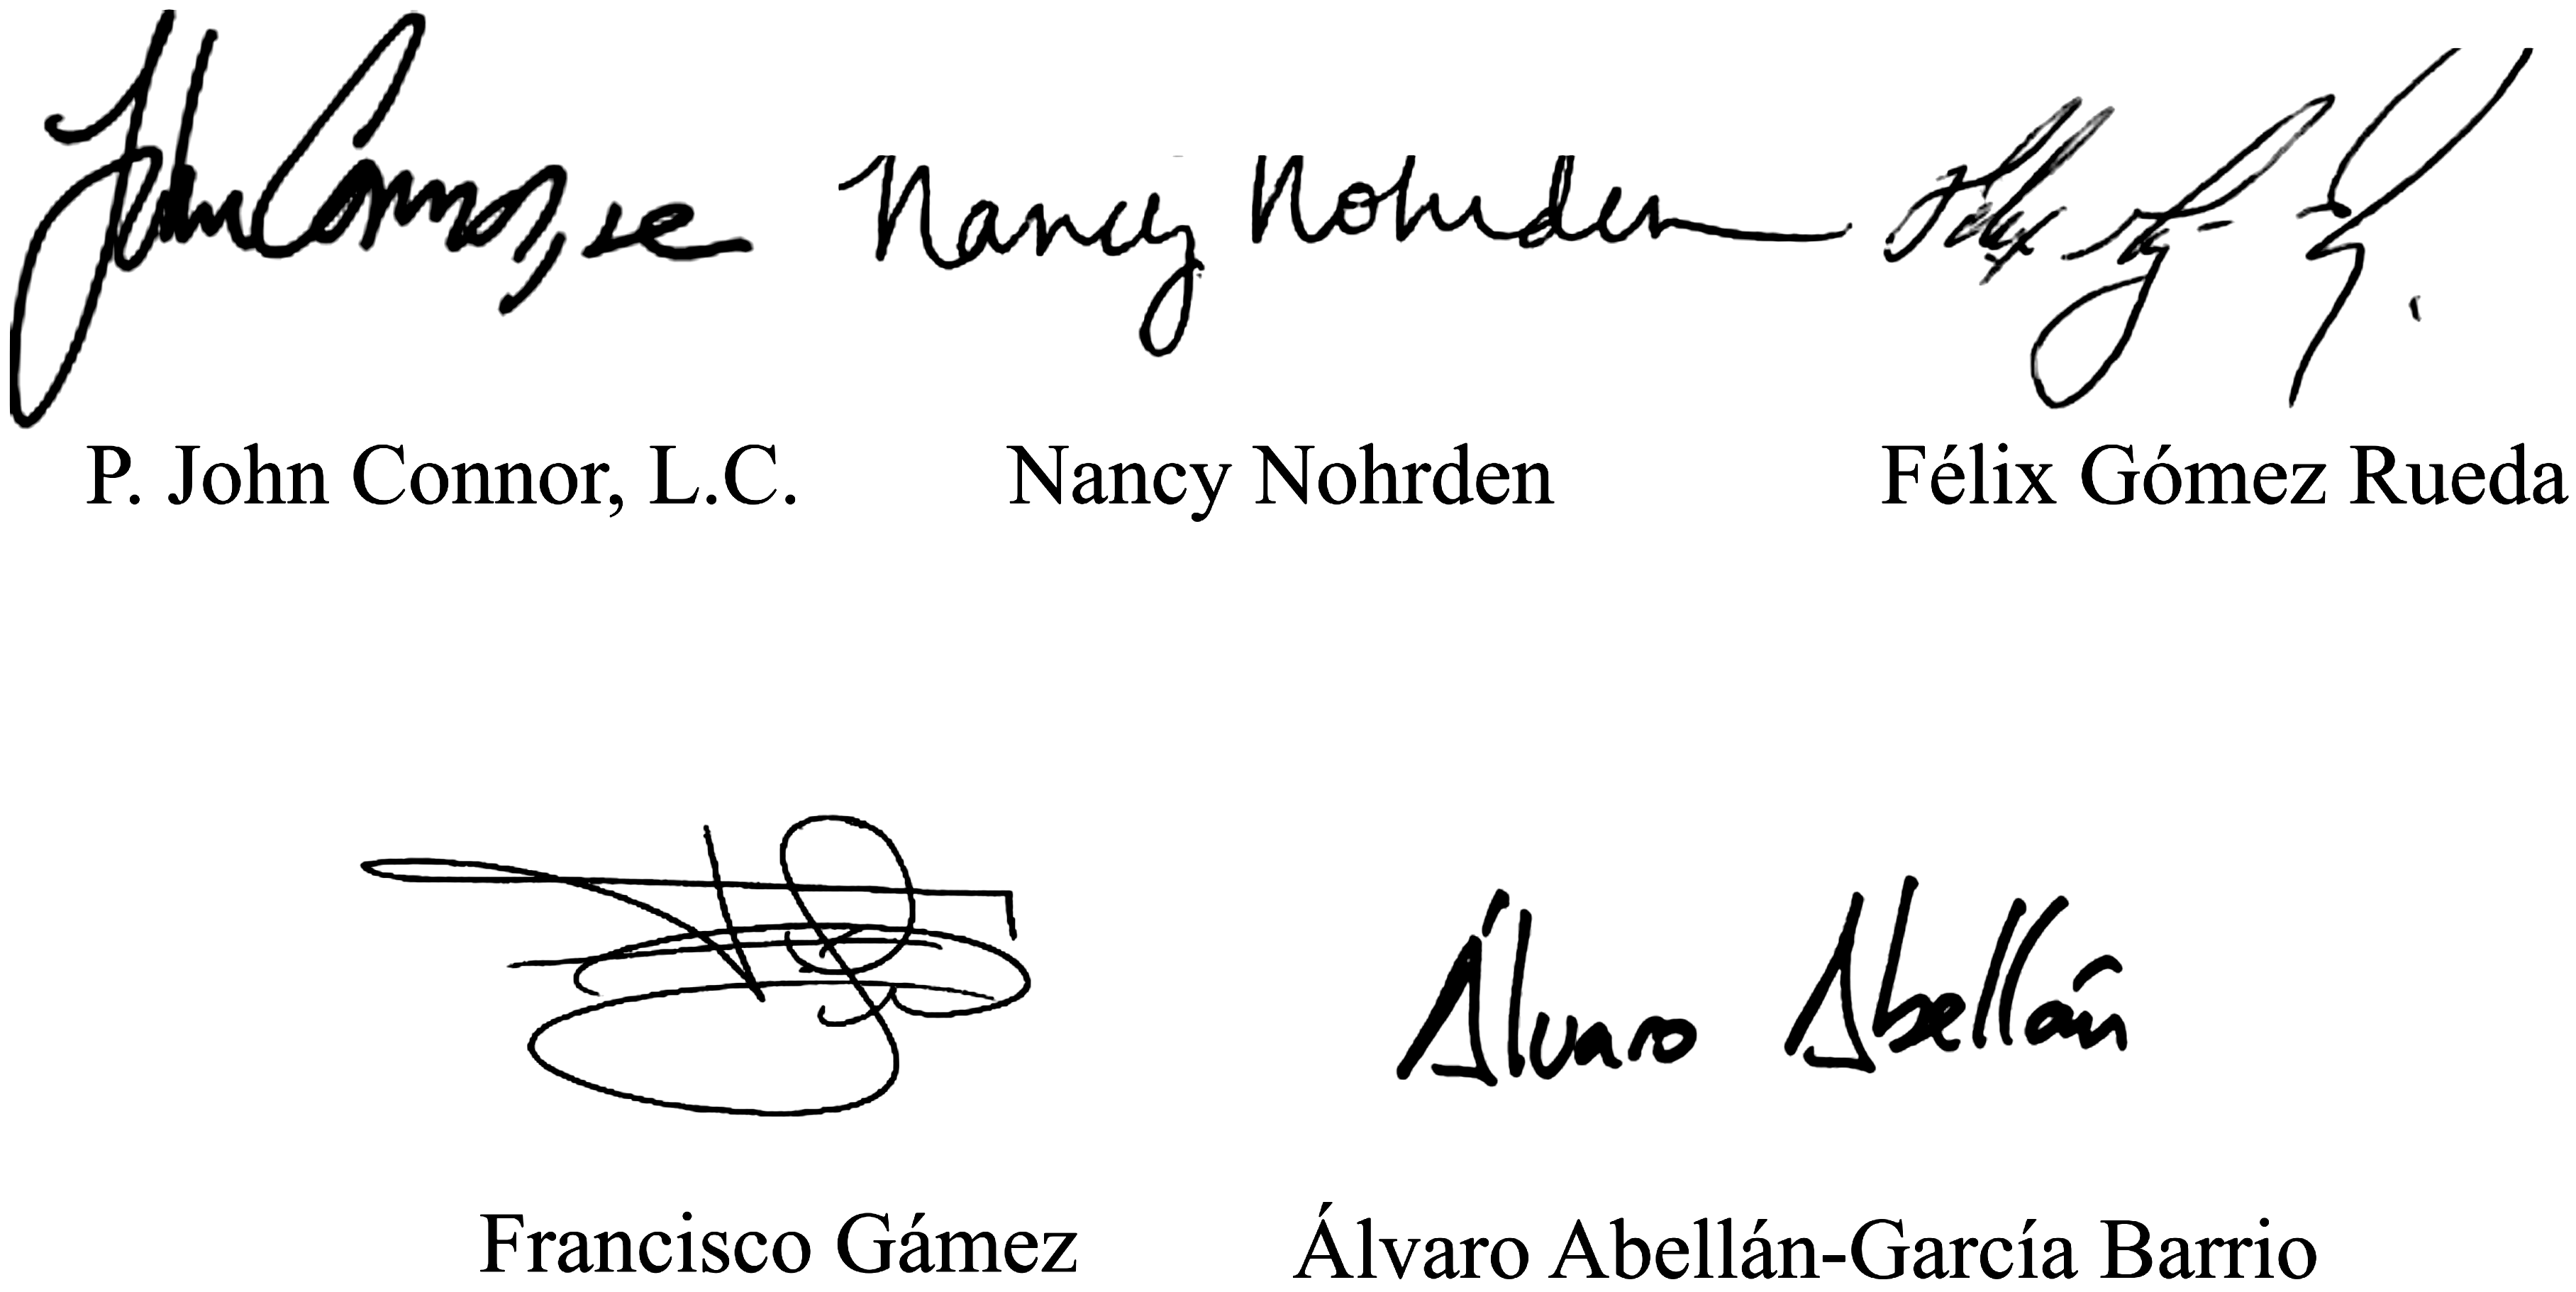
\includegraphics[width=\textwidth]{podpisy}
\end{center}








\setmainfont{HelveticaNeue}
\setlength{\parskip}{1em}
\setlength{\parindent}{0pt}


\cleardoublepage


\section*{Nota do polskiego tłumaczenia}


Tłumaczenie modlitewnika jest onieśmielającym zadaniem. Nie tylko bowiem należy oddać możliwie wiernie ducha oryginalnego tekstu, ale również trzeba zadbać, by modlitwy dobrze się odmawiało; by ich rytm i dobór słów odpowiadał polskiej tradycji. 


Dzięki zgłoszonym uwagom trzymasz w rękach drugie, poprawione wydanie polskiego tłumaczenia odnowionego modlitewnika świeckich członków Regnum Christi. Jesteśmy świadomi, że w dalszym ciągu mogły się w nim przemknąć błędy. Będziemy bardzo wdzięczni za wskazanie ich nam. Zarówno informacje o spostrzeżonych błędach, jak i propozycje ulepszeń można przesyłać na adres email 


\begin{center}
{\em modlitewnik2024@regnumchristi.pl}
\end{center}


Z góry dziękujemy!


Zespół tłumaczący




\cleardoublepage


\tableofcontents


\cleardoublepage


\gs{Wprowadzenie: „Panie, ucz nas modlitwy!”}


{\hnr Dzisiaj, w komunii z pierwszymi uczniami, kierujemy tę prośbę do Mistrza: „Panie, ucz nas modlitwy” (Łk 11, 1). W odpowiedzi Jezus uczy nas Modlitwy Pańskiej i opowiada nam przypowieść o natrętnym przyjacielu. Mówi nam, o co mamy się modlić i zachęca nas, abyśmy modlili się wytrwale, w porę i nie w porę, abyśmy otrzymali odpowiedź: „Proście, a będzie wam dane; szukajcie, a znajdziecie; kołaczcie, a otworzą wam. Każdy bowiem, kto prosi, otrzymuje, kto szuka, znajduje, a kołaczącemu otworzą” (Łk 11, 9-10). On włożył w nasze serca pragnienie modlitwy, modlitwy głębszej, przemiany naszego życia w modlitwę, liturgię; modlitwę nieustającą (por. Łk 18, 1-8), nie w sensie odmawiania modlitw co godzinę, ale w sensie życia wsłuchanego w Ducha Świętego, w obecności Boga, tak aby wszystkie nasze działania były odpowiedzią na Jego wolę, ofiarą dla naszego Pana.


Modlitwa w szkole Jezusa, w Kościele, jest codziennym sposobem spotykania Pana, z którym zawsze\linebreak idziemy i odpoczywamy. Jezus czeka na nas przy studni w najgorętszej i najsuchszej godzinie dnia, jako źródło wody, która nas zaspokaja. On mówi do nas: „Daj mi pić”, bo pragnie nas, a my, nawet jeśli o tym nie wiemy, pragniemy Boga: „Każdy, kto pije tę wodę, znów będzie pragnął, lecz kto pije wodę, którą Ja mu dam, nigdy pragnąć nie będzie, bo woda, którą Ja mu dam, stanie się w nim źródłem wody wytryskującej ku życiu wiecznemu” (J 4, 13-14).


Modlitewnik, który masz w swoich rękach -  „Panie, ucz nas modlitwy”, jest drogą inicjacji, wprowadzeniem do życia modlitwy, aby świeccy Regnum Christi uczyli się modlitwy modląc się, jako Kościół, w stylu Regnum Christi. Modląc się, jednoczymy się z modlitwą Chrystusa, z Jego Osobą i z Jego Ciałem - Kościołem, aby w łączności z Duchem Świętym zwracać się do Ojca. Posiadanie wspólnych modlitw i wskazówek pozwala nam rozpoznać, że jesteśmy włączeni w komunię Kościoła i Regnum Christi, nawet gdy modlimy się sami. Pomagają nam one również w czasie modlitwy wspólnotowej.}


\subsection*{Czym jest życie modlitwą?}
\fancyhead[RO]{\hnb\tiny Czym jest życie modlitwą?}




{\hnr Modlitwa nie jest czynnością autonomiczną, niezależną od reszty naszego życia. Poprzez życie modlitewne chcemy wyrazić dynamizm, który wypływa z osobistego spotkania z Chrystusem w liturgii i sakramentach, który umacnia się w naszych sercach poprzez nieustanną modlitwę i który rozlewa się, nadając aromat całemu naszemu światu. Chcemy także wyrażać nieustanne wsłuchiwanie się w Ducha Świętego, który stawia nam wyzwanie w sprawach naszego codziennego życia i wzbudza w naszych sercach odpowiedź, by przeżywać je tak, jak Chrystus gdy żył w ciele pośród nas.


Liturgia jest uprzywilejowaną przestrzenią spotkania\linebreak człowieka z Bogiem i Jego Synem, które objawia się poprzez znaki - czyny i słowa - wyraz dialogu i spotkania każdej osoby z Bogiem w Jego Kościele. Znajdziesz tu wskazówki dotyczące przeżywania niektórych sakramentów i wnoszenia ich jako „wody żywej” do modlitwy i codziennego życia. W szczególności znajdziesz odniesienia do okresów liturgicznych, sakramentów Eucharystii i Pojednania, wskazówki dotyczące\linebreak {\em Spotkania z Chrystusem} w twojej drużynie, a także obrzędu stowarzyszenia z Regnum Christi, abyś mógł lub mogła zawsze odnawiać ten kamień milowy w swojej historii miłości do Boga i przynależności do Regnum Christi.


Życie modlitewne obejmuje konkretne momenty, którym towarzyszą zewnętrzne znaki. Znaki te pomagają nam modlić się również ciałem, pozwalając modlitwie dotrzeć do całej naszej istoty i działania, uświęcając je. Życie modlitwy, karmione sakramentami, zwalcza zatwardziałość naszego serca (por. Ps 95, 8), pozwalając by to Chrystus, a nie my, w nim królował (por. Ga 2, 20). Znajdziesz tu wiele modlitw, które są tradycją Kościoła, takich jak {\em Ojcze nasz}; ale są też te szczególne dla Regnum Christi.


Wreszcie, życie modlitewne jest „przedłużeniem” sakramentów czyniącym z nas żywą liturgię, wyrażającą się w wielu znakach obecność Królestwa Chrystusa: współczucie dla najbardziej potrzebujących, komunia z naszymi braćmi i siostrami, dzieła miłości i miłosierdzia, świadectwo i misja, nowe sposoby przeżywania małżeństwa, rodziny i pracy, nowa kultura.


To właśnie obecność Królestwa karmi tę duchowość, dzięki której powracamy do liturgii, sakramentów i modlitwy, starając się „przyoblec w Chrystusa w naszych sercach i czynach, aby mógł On królować w naszym życiu poprzez stopniowe upodabnianie się do Niego”, pozwalając się „przeniknąć miłością Chrystusa do ludzi”, aby „mógł On królować w sercach wszystkich ludzi i w społeczeństwie” (SFRC 13). Kulminacją takiego stylu życia jest adoracja.}


\subsection*{Jaka jest struktura niniejszego modlitewnika?}
\fancyhead[RO]{\hnb\tiny Jaka jest struktura niniejszego modlitewnika?}


{\hnr Przyroda i ludzkie życie mają swój rytm dzienny, tygodniowy i roczny. Liturgia towarzyszy temu rytmowi, ucząc nas dostrzegać niewidzialną obecność Królestwa w zwykłym czasie natury i życia. Istnieją modlitwy i gesty, które powtarzamy codziennie, inne co tydzień, a jeszcze inne w określonych porach roku. Często obchodzimy jeden dzień w roku, aby w wyjątkowy sposób pamiętać o tym, co jest ważne w każdej godzinie naszego życia. W ten sposób modlitwa staje się nawykiem, a nawyk modlitewnym życiem.


Duża część niniejszego modlitewnika odpowiada tej naturalnej i liturgicznej strukturze: dzień, tydzień i rok,\linebreak a wszystkie biorą swój początek w dniu ósmym, niedzieli, Dniu Pańskim. Ale życie jest również naznaczone wyjątkowymi okazjami, wyjątkowymi sytuacjami\linebreak o szczególnym znaczeniu dla nas. Na końcu znajdziesz modlitwy i wskazówki dotyczące takich wydarzeń.}


\vspace{\fill}


\subsection*{Jak najlepiej wykorzystać niniejszy modlitewnik?}
\fancyhead[RO]{\hnb\tiny Jak najlepiej wykorzystać niniejszy modlitewnik?}


{\hnr Oto siedem sprawdzonych wskazówek, jak wzrastać w życiu modlitewnym:


\begin{itemize}


\item Postaw się w obecności Boga, uświadom sobie, co zamierzasz robić, przygotuj swoje serce. Szukaj wewnętrznej i zewnętrznej ciszy. Staraj się modlić z sensem i wszystkimi zmysłami. Poproś Ducha Świętego, aby prowadził twój umysł i wypełniał twoje serce.


\item Zwróć się ku Słowu Bożemu, Pismu Świętemu, które jest nieustannym dialogiem między Bogiem a człowiekiem. Nie ma lepszego sposobu na rozpoczęcie naszego życia modlitewnego niż uczenie się od Tego, który modli się najlepiej, czyli od Niego. Staraj się modlić z takimi samymi uczuciami jak Jezus: niech Chrystus będzie tym, który żyje, działa i modli się w tobie.


\item Kontempluj słowa i znaki liturgii, uprzywilejowanego miejsca spotkania Boga z Jego ludem,\linebreak gdzie działanie Boga łączy się z działaniem człowieka w doskonałej synergii.


\item Od czasu do czasu medytuj nad modlitwami ustnymi. Są one wyrazem wiary, ale także ją odżywiają. Naucz się delektować i odnawiać ich znaczenie, odnosząc je do swojego życia. Staraj się pamiętać nie tylko literę, ale także ducha. Pamiętać, to wracać przez serce.


\item Pozwól się Jemu prowadzić: nie chodzi o to, co robimy w modlitwie, ale o to, co On chce w nas uczynić. Można nic nie czuć, nie znaleźć odpowiedzi, a mimo to dobrze się modlić. Chociaż „nie umiemy się modlić tak, jak trzeba” (Rz 8, 26), On to wie i jest z nami.


\item Wejście w modlitwę może trochę potrwać. Nic nie szkodzi. Milcz i słuchaj Jego Słowa. Zdarza się, że możesz ulec rozproszeniu. Nie jest to niczym niezwykłym. Nie rób z tego wielkiej sprawy. Spróbuj wrócić do modlitwy.


\item Przed zakończeniem postaraj się, aby modlitwa ożyła. Wyobraź sobie małe postanowienie, które możesz wkrótce zrealizować, które jest proste, realistyczne i stanowcze.


\end{itemize}


Wszystkiego tego można się nauczyć poprzez osobistą praktykę, rady bardziej doświadczonych ludzi i modlitwę dzieloną z innymi. Poproś swojego kierownika duchowego o radę, poszukaj nauczycieli i partnerów modlitwy, postaraj się, aby Spotkanie z Chrystusem w twoim zespole stało się szkołą modlitwy. W czwartej części Katechizmu, „O modlitwie chrześcijańskiej”, znajdziesz bardzo proste i wyczerpujące wprowadzenie do życia modlitwy.


Często w rubrykach - tekstach w kolorze czerwonym - można znaleźć zaproszenie do pójścia głębiej, do pogłębienia początków, które tutaj oferujemy. W życiu modlitwy są etapy, ale te późniejsze nie przekreślają pierwszych. Oto kilka wskazówek, które mogą ci zawsze towarzyszyć, ale życie Ducha nie kończy się na tych stronach.


„Modlisz się tym, kim jesteś”, ufając, że staniesz się tym, o co się modlisz. Modlimy się tak, jak żyjemy i żyjemy tak, jak się modlimy. Sposób, w jaki się modlisz, zmieni się wraz z tobą. Chociaż dźwięki modlitw ustnych pozostają, Duch odnawia je i sprawia, że wypływają z nich rzeki wody żywej. Prośmy o ten dar, który Pan chce nam dać.}


\gs{Niedziela, dzień ósmy}


{\hnr Niedziela stanowi centrum życia Kościoła. Jest pierwszym dniem tygodnia, pamiątką pierwszego dnia stworzenia, a także ósmym dniem, w którym Chrystus przez swoje Zmartwychwstanie doprowadza szabat do jego wypełnienia i wykonania. Czas chronologiczny,\linebreak w którym wszystko, co się rodzi, umiera, zostaje przekroczony przez czas przemieniony, który uczestniczy w wieczności. Niedziela wyznacza początek nowego czasu i nowej przestrzeni: życia w Królestwie.


W niedzielę ćwiczymy szczególnie, jak przeżywać każdy dzień roku w święty sposób. Jest to dzień świętowania i odpoczynku; dzień rodzinny, kulturalny i społeczny; dzień liturgii i modlitwy par excellence. Kościół nakazuje obowiązkowe uczestnictwo wiernych w niedzielnej liturgii, ale także usilnie zachęca do częstszego, nawet codziennego uczestnictwa w Eucharystii, jako uprzywilejowanego sposobu, aby Chrystus był\linebreak wszystkim we wszystkich.}


\vspace{\fill}




\gss{Eucharystia}


{\hnr Eucharystia jest sakramentem sakramentów, źródłem\linebreak i szczytem całego życia chrześcijańskiego. W niej łączy się całe duchowe dobro Kościoła: z jednej strony sam Chrystus zostaje sprowadzony na ziemię, a przez Jego wcielenie, śmierć i zmartwychwstanie świat zostaje uświęcony; z drugiej strony nasze uwielbienie, modlitwa i wyrzeczenia, w Duchu Świętym, wznoszą nas ku niebu i docierają do Chrystusa i Ojca. Nasze myśli\linebreak i uczucia, nasze słowa i czyny są inspirowane, potwierdzane i wzmacniane przez Eucharystię.


Eucharystia jest pamiątką ofiary Chrystusa i Jego Ciała, którym jest Kościół. Jedyna ofiara Chrystusa aktualizuje się i uobecnia skutecznie w każdej Eucharystii; ofiara wiernych jednoczy się z nią, zyskując w ten sposób nową wartość wstawiennictwa za całe stworzenie. Poprzez działanie Chrystusa i odpowiedź Kościoła Eucharystia odnawia centrum historii zbawienia.


Eucharystia jest nazywana różnymi imionami, podkreślającymi różne aspekty jej niewyczerpanego bogactwa. Warto zastanowić się nad znaczeniem każdej\linebreak z nich. Niektóre z nich to: Eucharystia, jako dziękczynienie i uwielbienie; uczta Pańska, jako ostatnia wieczerza Chrystusa z uczniami i przedsmak uczty weselnej Baranka w niebieskim Jeruzalem; pamiątka męki i zmartwychwstania Pana; święta i boska liturgia, ponieważ jest centrum i najgłębszym wyrazem świętego życia; komunia, ponieważ prowadzi do zjednoczenia między Chrystusem a Jego Kościołem; Msza święta, ponieważ celebracja tajemnicy zbawienia osiąga punkt kulminacyjny w posłaniu lub misji wiernych do wypełnienia woli Bożej w codziennym życiu.}


\gss{Przygotowanie do Eucharystii}


{\hnr Eucharystia jest wielkim świętem. Jak wszystkie uroczystości, rozpoczyna się od ekscytujących przygotowań, zawiera własne obrzędy i pozostaje z nami po jej zakończeniu.
Przed pójściem na Eucharystię powinniśmy przygotować nasze umysły i serca. Być może powinniśmy przystąpić do sakramentu pojednania, a także zawrzeć pokój z naszymi braćmi i siostrami, aby nic nie ciążyło nam na sercu, gdy Chrystus przyjdzie się\linebreak z nami spotkać. Możemy również zadać sobie pytanie, dlaczego lub za kogo ofiarujemy Mszę św. i co duchowo złożymy w ofierze razem z chlebem i winem, aby Chrystus napełnił je swoim życiem i uczynił świętymi. O co chcemy prosić Pana? Co chcemy dać Panu, aby mógł to uświęcić i włączyć do swojego Królestwa?}


\gss{Celebracja Eucharystii}


{\hnr Obrzędy wstępne są częścią przygotowania: przemieniają przestrzeń, czas i serce oraz gromadzą wiernych i Chrystusa, niewidzialną głowę Kościoła. Wejście; pozdrowienie ołtarza i ludu przez kapłana; znak krzyża, przez który odnawiamy nasz chrzest i nasze uczestnictwo w wiecznej rodzinie (Ojciec, Syn i Duch Święty); akt pokutny i pieśń miłosierdzia, przez które uznajemy się za osądzonych i zbawionych; Gloria, w którym niebo zostaje otwarte i słyszymy aniołów ogłaszających Wcielenie; oraz modlitwa kolekty, która kładzie nacisk na znaczenie celebracji.


Liturgia Słowa objawia Pana, który wychodzi nam na spotkanie. Jest to poryw miłości, poprzez który Ojciec daje nam swoje Słowo, aby obudzić naszą wiarę i oczekuje, że je przyjmiemy i ożywimy. Czytanie Słowa czyni nas oblubienicą Baranka: słuchając i przyjmując Słowo, stajemy się Jego ciałem. On nas wzywa, czy odpowiemy?


Podczas ofiarowania darów (offertorium) kapłan w imieniu Chrystusa ofiaruje chleb i wino Ojcu, aby Chrystus przemienił je w swoje Ciało i Krew. Wraz z kapłanem, przy chlebie i winie, składamy nasze modlitwy, cierpienia i uczynki, aby Chrystus mógł włączyć je do Królestwa. Tylko On może doprowadzić do doskonałości wszystkie ludzkie próby składania ofiar.


Liturgia eucharystyczna jest sercem i zwieńczeniem celebracji: chleb i wino stają się Ciałem i Krwią Jezusa Chrystusa. Uczestnicząc w komunii, przyjmujemy samego Chrystusa, który oddał się za życie świata. Obrzęd komunii kończy się wielką ciszą.


Msza kończy się rozesłaniem, misją: wnieść nowe życie przemienione przez Chrystusa w życie osobiste, rodzinne, społeczne, zawodowe i kulturowe. „Idźcie\linebreak w pokoju! Chwalmy Pana naszym życiem! Niech radość Pana będzie naszą siłą!”}


\gss{Modlitwy w czasie Eucharystii}


{\hnr Liturgia eucharystyczna jest pełna czynności, słów, modlitw i pieśni, które razem wzięte wyrażają niewyczerpane bogactwo naszej intymnej relacji z Chrystusem, z Ojcem i z Duchem Świętym. Cisza jest również znakiem: oczekiwania, skruchy, słuchania, uwielbienia,\linebreak  chwały, adoracji, dziękczynienia. Cisza pomaga nam zmierzyć się z tym, co już się wydarzyło i przygotować się na to, co ma nadejść. Tradycja mówi szczególnie\linebreak o wielkiej ciszy lub świętej ciszy po komunii, w której Kościół zaleca, aby nie śpiewać, aby Słowo, Liturgia i poruszenia, które otrzymaliśmy, mogły odbijać się\linebreak w nas echem.


Mamy modlitwy, które pomagają nam przygotować się przed Eucharystią, inne, aby zintensyfikować nasze\linebreak uczucia eucharystyczne, a jeszcze inne, aby modlić się\linebreak w określonych momentach celebracji. Biorąc pod uwagę bogactwo sakramentu i zalecenia Kościoła,\linebreak z jednej strony, oraz etap i stan naszego życia duchowego, z drugiej strony, możemy rozeznać, z pomocą naszego kierownika duchowego, stosowność korzystania z niektórych z tych modlitw od czasu do czasu.


Wielu wiernych pozostaje w kościele po Mszy Świętej na krótką chwilę osobistej, spontanicznej lub śpiewanej modlitwy. Tradycją niektórych wspólnot Regnum Christi jest modlitwa za papieża i o powołania na zakończenie Eucharystii.}










\gs{Dzień, który jest modlitwą}




{\hnr „Dzień dniowi głosi opowieść, a noc nocy przekazuje wiadomość.” (Ps 19, 3). Bóg przemawia do nas w każdej godzinie i zaprasza nas do rozmowy z Nim i ofiarowania Mu wszystkiego, czego doświadczamy. W ten sposób dzień i noc stają się nieustanną modlitwą.


O świcie otwieramy oczy z przebudzonym sercem (por. Ps 57, 9), otwarci na Pana, który wychodzi nam na spotkanie w codzienności, w każdych okolicznościach, pośród trosk tego życia (por. Mt 6, 34). Jesteśmy wdzięczni za dar nowego dnia i ofiarujemy Panu nasze sprawy.


Poświęcamy kilka minut na modlitwę, aby przypomnieć sobie, że każda minuta dnia jest modlitwą. Medytacja, pozdrowienie Matki Bożej, różaniec, nawiedzenie Eucharystii i komunia duchowa są okazjami do odzyskania i przedłużenia życia modlitwy pośród świata.


Schyłek dnia przypomina zmierzch życia i oznacza jego koniec. Jest to czas na podsumowanie, dziękczynienie Bogu i powierzenie wszystkiego, czego doświadczyliśmy, Jego miłosierdziu (por. Ps 32). Temu właśnie poświęcamy nasze wieczorne modlitwy.


Sen i czuwanie, praca i wypoczynek, przyjaciele i rodzina... wszystko należy do Boga, jest okazją do rozpoznania Jego obecności, głoszenia jej i życia w Królestwie.}


\gss{Po przebudzeniu}


{\hnr Prośba o Bożą obecność o poranku pomaga nadać ton całemu dniu i sens życiu. Przebudzić się to narodzić się na nowo, żyć z nowym sercem i nowym duchem. Jest to czas, aby wznieść nasze umysły i serca do Pana\linebreak i poprosić Go, aby zstąpił do naszego życia, aby je dotknął i obudził.}


{\hnr\strong{Wezwanie}}


Chryste nasz Królu! Przyjdź Królestwo Twoje!


{\hnr Następnie odmawiamy {\em Ojcze nasz}, {\em Zdrowaś Maryjo},\linebreak po których następują:}


{\hnr\strong{Prośba na początek dnia}}


Mój Panie i mój Ojcze, natchnij moje myśli, słowa i działania, i dopomóż mi, aby wszystko, co będę czynić rozpoczynało się i kończyło zgodnie z Twoją wolą i z miłości ku Tobie. Przez Chrystusa, Pana naszego. Amen.


\gss{Ofiarowanie dnia}


{\hnr Ofiarowanie naszych działań jest znakiem ofiarowania naszego życia. Chodzi o to, abyśmy się stali darem\linebreak z siebie. Proponujemy trzy modlitwy ustne do Boga\linebreak i jedną do Najświętszej Maryi Panny. Rozpoczynają się one od uczynienia znaku krzyża, aby stanąć w obecności Pana. Pomocne może okazać się włączenie własnej modlitwy. Modlitwy ofiarowania można zastąpić {\em Jutrznią} z Liturgii Godzin. W obu przypadkach zachęcamy do odmawiania {\em Modlitwy do Jezusa Chrystusa}, która jest wspólna dla wszystkich członków Regnum Christi.}


W imię Ojca i Syna, i Ducha Świętego. Amen.


{\hnr\strong{Modlitwa do Boga Ojca}}


Wierzę w Ciebie, mój Boże, ponieważ jesteś samą\linebreak prawdą. Pokładam w Tobie nadzieję, ponieważ jesteś nieskończonym miłosierdziem. Kocham Cię ponad\linebreak wszystko, ponieważ jesteś nieskończenie łaskawy i ponieważ tylko Ciebie muszę kochać z całego serca,\linebreak z całej duszy i ze wszystkich sił (por. Pwt 6, 5). Dziękuję Ci, Ojcze, że dałeś mi nowy dzień, abym oddał(a) Ci chwałę i uobecnił(a) Twoje Królestwo. Amen


\filbreak{\hnr\strong{Modlitwa do Jezusa Chrystusa}}


Panie Jezu, oddaję Ci moje ręce, by pracować dla Ciebie. Oddaję Ci moje stopy, by podążać Twą drogą. Oddaję Ci moje oczy, by widzieć tak jak Ty widzisz. Oddaję Ci moje usta, by wymawiać Twe słowa. Oddaję Ci mój umysł, byś Ty myślał we mnie. Oddaję Ci mego ducha, byś Ty się we mnie modlił. Przede wszystkim oddaję Ci moje serce, byś we mnie kochał swego Ojca i wszystkich ludzi. Oddaję Ci całą mą osobę, byś Ty we mnie rósł, byś to Ty, Jezu, był tym, który żyje, pracuje i modli się we mnie. Amen


{\hnr\strong{Modlitwa do Ducha Świętego}}


Duchu Święty, łagodny gospodarzu i pocieszycielu mojej duszy, przewodniku i mistrzu naszej przemiany\linebreak w Chrystusie: oświeć mój rozum, abym poznał(a) Twoją wolę; rozpal moje serce, abym kochał(a) ją z pasją\linebreak i udziel mi niezbędnej siły, abym ją wypełnił(a) tak, jak mnie o to prosisz. Daj mi, Duchu miłości, łaskę wiernej odpowiedzi na Twoje święte natchnienia. Amen.


{\hnr\strong{Modlitwa do Najświętszej Maryi Panny}}


Matko moja, przychodzę do Ciebie w tym nowym dniu, aby poświęcić Ci wszystkie moje myśli, słowa i czyny oraz prosić o błogosławieństwo dla mnie, moich bliskich i wszystkich ludzi, których Bóg postawił na mojej drodze. Wyproś mi serce apostoła Królestwa i pomóż mi naśladować życie modlitwy, posłuszeństwa, pokory, wierności, poświęcenia i prostoty, które dzieliłaś ze swoim Synem, naszym bratem i Panem. Powiedz Jezusowi, Matko, że chcę Mu służyć w Regnum Christi, aby Jego Królestwo było obecne wśród ludzi. Amen.


{\hnr\strong{Planowanie dnia}}


{\hnr Poświęćmy kilka minut na refleksję w obecności Boga, aby przejrzeć plan dnia, ofiarować Mu nasze działania i odnowić nasz cel życia w Chrystusie na  cały dzień.}


\gss{Medytacja}




{\hnr Medytacja lub „modlitwa myślna” ułatwia intymny i osobisty dialog z Bogiem. Podobnie jak Jezus, potrzebujemy się modlić, rozmawiać z naszym Ojcem i słuchać Go. Czynić to jako synowie w Synu, z Duchem Świętym, który przychodzi, aby pomóc nam w naszej słabości, ponieważ nie wiemy, jak się modlić (por. Rz 8, 26).


Słowo Boże musi być obecne w naszej modlitwie, czy to jako temat medytacji, czy w rozmowie z Panem. Pomyślmy o tym, jak modlili się uczniowie z Emaus i jak płonęły ich serca, gdy słuchali Pana: jak Jezus doprowadził ich do refleksji nad ich troskami i do znalezienia w Piśmie Świętym klucza do interpretacji ich życia (por. Łk 24, 13-35).


Nie wystarczy rozmyślać i kontemplować. Medytacja jest uważnym i pełnym miłości dialogiem z Bogiem. Trzeba zatem nauczyć się słuchać Boga w ciszy swojej duszy i rozmawiać z Nim w pełni wiary i miłości, aby wejść z Nim w osobisty kontakt. To właśnie w tym momencie, pod wpływem światła i mocy Ducha Świętego, własna wola dostosowuje się do woli Bożej i podejmowane są decyzje, które kierują naszym życiem.


Modlitwa rozpoczyna się znakiem krzyża i wezwaniem do Ducha Świętego; kontynuuje się ją aktami przygotowawczymi, które pomagają nam wejść w synergię\linebreak z Bogiem, aby mieć te same uczucia, co modlący się Jezus. Pod koniec modlitwy dziękujemy Panu za spędzony z Nim czas i za otrzymane owoce, które zawsze są większe niż te dostrzegalne. Wreszcie, prosimy\linebreak o Jego łaskę, aby zanieść innym to, co On nam dał.}


\filbreak{}W imię Ojca i Syna, i Ducha Świętego. Amen.


\filbreak{\hnr Wezwanie do Ducha Świętego}


{\hnr P:} Przyjdź Duchu Święty\\
{\hnr W:} Napełnij serca Twoich wiernych i rozpal w nich ogień Twojej miłości. 


{\hnr P:} Ześlij nam Ducha Stworzyciela\\
{\hnr W:} I odnów oblicze ziemi.


{\hnr P:} Boże, Ty, który oświeciłeś nasze serca światłem Ducha Świętego daj nam w tymże Duchu poznać, co jest prawe i Jego pociechą zawsze się radować. Przez Chrystusa, Pana naszego. \\
{\hnr W:} Amen.


{\hnr {\strong{Akty przygotowawcze: akt wiary, nadziei i miłości}}


Akty te są podejmowane w bezpośrednim dialogu\linebreak z Bogiem, w sposób krótki i spontaniczny, bez potrzeby korzystania ze spisanych formuł. Wprowadzają nas one w modlitwę, ponieważ same w sobie są istotną treścią modlitwy, która polega na wierze, nadziei i miłości. Wskazujemy kilka ewangelicznych słów i obrazów, które mogą być pomocne, choć każdy odnajduje swoje własne i zmienia je w miarę robienia postępów w serdecznej relacji z Bogiem i Jego Słowem.


Wiara: bądź świadomy, że jesteś w obecności wszechmogącego Boga, rozmawiając z Nim -  „Ojcze nasz”.\linebreak Być może pamiętasz ten moment, w którym Jezus mówi do niedowierzającego Tomasza: „Podnieś tutaj swój palec i zobacz moje ręce. Podnieś rękę i włóż [ją] do mego boku, i nie bądź niedowiarkiem, lecz wierzącym!”. Na co Tomasz odpowiada słowami, które wyrażają jego odnowioną wiarę: „Pan mój i Bóg mój” (J 20, 27-28).


Nadzieja: zaufanie Bogu jako najwyższemu dobru, twojemu Zbawicielowi, od którego z ufnością oczekujemy łaski i pomocy w naszej nędzy. „Przyjdź Królestwo Twoje”. Być może przypominasz sobie moment, w którym syn marnotrawny powraca do domu ojca, a ten wita go przedsmakiem życia w Królestwie: „Przynieście szybko najlepszą szatę i ubierzcie go; dajcie mu też pierścień na rękę i sandały na nogi! Przyprowadźcie utuczone cielę i zabijcie: będziemy ucztować i bawić się, ponieważ ten mój syn był umarły, a znów ożył; zaginął, a odnalazł się”. (Łk 15, 22-24).


Miłość: uświadom sobie, że Bóg jest twoim Ojcem, a ty jesteś Jego ukochanym dzieckiem. Zwróć się do Niego jak syn do ojca i słuchaj Go. „Bądź wola Twoja. Chleba naszego powszedniego daj nam dzisiaj. Odpuść nam nasze winy, jako i my odpuszczamy naszym winowajcom”.


Możesz przypomnieć sobie chwile braterskiej wspólnoty między Jezusem a Jego uczniami; lub Betanię,\linebreak w domu Łazarza; lub nadrzędny moment Jego skrajnego oddania siebie, z Marią i Janem, u stóp Krzyża.


Proś Chrystusa i Maryję o pomoc, aby medytacja była owocna.


Na zakończenie medytacji podziękuj Bogu. Możesz\linebreak użyć modlitwy końcowej.}




\gss{Pozdrowienie Najświętszej Maryi Panny}


{\hnr Maryja towarzyszy nam przez cały dzień poprzez cichą obecność matki. Kierujemy do Niej nasze modlitwy\linebreak w określonych porach dnia, zwłaszcza odmawiając\linebreak {\em Anioł Pański}, {\em Regina Cæli} i Różaniec.


Anioł Pański i Regina Cæli to mała liturgia godzin, którą Kościół zaleca tym, którzy nie mają czasu na przerwanie swoich zajęć. Przez kilka minut, zwykle w południe, wspominamy z Maryją niektóre tajemnice z życia Chrystusa.}


{\hnr\strong{Anioł Pański}}


{\hnr Anioł Pański jest odmawiany przez cały rok, z wyjątkiem okresu Wielkanocnego.}


{\hnr P:} Anioł Pański zwiastował Pannie Maryi.\\
{\hnr W:} I poczęła z Ducha Świętego.


{\hnr P:} Zdrowaś Maryjo, łaski pełna, Pan z Tobą, błogosławionaś Ty między niewiastami, i błogosławiony owoc żywota Twojego, Jezus. \\
{\hnr W:} Święta Maryjo, Matko Boża, módl się za nami grzesznymi teraz i w godzinę śmierci naszej. Amen


{\hnr P:} Oto ja służebnica Pańska.\\
{\hnr W:} Niech mi się stanie według słowa Twego.


{\hnr P:} Zdrowaś Maryjo…


{\hnr P:} A Słowo ciałem się stało.\\
{\hnr W:} I zamieszkało między nami.


{\hnr P:} Zdrowaś Maryjo…


{\hnr P:} Módl się za nami, Święta Boża Rodzicielko.\\
{\hnr W:} Abyśmy się stali godnymi obietnic Chrystusowych.


{\hnr P:} Módlmy się: Prosimy Cię, Panie, wlej w nasze serca swoją łaskę, abyśmy, poznawszy za Zwiastowaniem Anielskim wcielenie Chrystusa Syna Twojego, przez Jego mękę i krzyż zostali doprowadzeni do chwały zmartwychwstania. Przez Chrystusa Pana naszego. 


{\hnr W:} Amen.


{\hnr P:} Chwała Ojcu i Synowi, i Duchowi Świętemu.\\
{\hnr W:} Jak była na początku, teraz i  zawsze, i  na wieki wieków. Amen. (Trzy razy)


{\hnr\strong{Regina Cæli}}


{\hnr Regina Cæli jest odmawiana w okresie wielkanocnym: od Niedzieli Wielkanocnej do południa w sobotę Zesłania Ducha Świętego.}


{\hnr P:} Królowo nieba, wesel się, alleluja


{\hnr W:} Bo Ten, któregoś nosiła, alleluja\\
Zmartwychwstał jak powiedział, alleluja\\
Módl się za nami do Boga, alleluja\\
Raduj się i wesel, Panno Maryjo, alleluja\\
Bo zmartwychwstał Pan prawdziwie, alleluja


{\hnr P:} Módlmy się: Boże, któryś przez zmartwychwstanie Syna swojego, Pana naszego Jezusa Chrystusa świat uweselić raczył, daj nam, prosimy, abyśmy przez Jego Rodzicielkę Pannę Maryję dostąpili radości życia wiecznego. Przez tegoż Chrystusa Pana naszego.


{\hnr W:} Amen.


{\hnr P:} Chwała Ojcu i Synowi, i Duchowi Świętemu.\\
{\hnr W:} Jak była na początku, teraz i  zawsze, i  na wieki wieków. Amen. (Trzy razy)


{\hnr\strong{Modlitwa do Anioła Stróża}}


{\hnr W Regnum Christi mamy zwyczaj powierzać się Aniołowi Stróżowi na zakończenie modlitwy Anioł Pański lub Regina Cæli.}


Aniele Boży Stróżu mój\\
Ty zawsze przy mnie stój\\
Rano, wieczór, we dnie, w nocy\\
bądź mi zawsze do pomocy\\
Strzeż duszy, ciała mego\\
zaprowadź mnie do żywota wiecznego\\
Amen


{\hnr lub}


Aniele Pański, mój wierny opiekunie; ponieważ Boża Opatrzność powierzyła mnie Tobie, oświecaj mnie\linebreak i strzeż, umocnij mnie i kieruj mną. Amen


{\hnr lub}


Aniele Pański, który prowadzisz mnie, badź moim światłem i krocz obok mnie. Bądź moim obrońcą i ochraniaj mnie, po ścieżkach życia prowadź mnie. Amen.






\gss{Różaniec}


{\hnr Odmawianie różańca jest modlitwą typowo medytacyjną. Zapoczątkowana na Zachodzie przez chrześcijan, odpowiada w pewien sposób modlitwie serca lub modlitwie Jezusowej, typowej dla chrześcijańskiego\linebreak Wschodu. Regnum Christi zachęca ludzi do odmawiania przynajmniej jednej tajemnicy różańca każdego\linebreak dnia, w grupie lub prywatnie.


Różaniec to czas, w którym Maryja jest obecna w naszym życiu, dając nam pocieszenie, przykład i wstawiennictwo. Modlitwa ta przynosi pokój duszy, zaszczepia wiarę i odnawia ufność.


Podczas odmawiania {\em Ojcze nasz}, {\em Zdrowaś Maryjo}\linebreak i {\em Chwała Ojcu}, recytowane są tajemnice życia, śmierci, męki i zmartwychwstania Chrystusa, widziane oczami Matki Bożej. W ten sposób pozwalamy Matce Bożej formować nas w uczuciach Serca Jej Syna. Zdarza się, że podczas odmawiania różańca możemy ulec rozproszeniom; wystarczy podjąć modlitwę z ufnością i spróbować na nowo wydobyć jej znaczenie, pamiętając o~tajemnicach, które celebrujemy i o ludziach, za których się modlimy.}


\filbreak{\hnr\strong{Różaniec odmawiany w grupie}}


{\hnr Gdy różaniec jest odmawiany w grupie, rozpoczyna go prowadzący, który zapowiada każdą z tajemnic i intencję ogólną; pięciu uczestników może przedstawić intencje, w których grupa chce ofiarować każdą z tajemnic.}


{\hnr P:} W imię Ojca i Syna, i Ducha Świętego. Amen.


{\hnr P:} Panie mój, Jezu,\\
{\hnr W:} Boże i prawdziwy człowiecze, Stworzycielu i Zbawicielu mój. Ponieważ jesteś „Tym, który jesteś”, i ponieważ kocham Cię ponad wszystko, z całego serca żałuję, że Cię obraziłem. Pragnę i postanawiam wyspowiadać się wkrótce. Ofiarowuję moją pracę, moje czyny i moje życie jako zadośćuczynienie za moje grzechy. Ufam Twej dobroci i Twemu nieskończonemu Miłosierdziu, że mi przebaczysz i dasz mi tę łaskę, abym cię już więcej nie obrażał. Amen.


{\hnr P:} Ofiarujemy ten różaniec za/o…


{\hnr Po każdym fragmencie biblijnym jeden z uczestników może wypowiedzieć swoją intencję.}


\filbreak{\hnr Tajemnice radości (poniedziałek i sobota)}


{\hnr P:} Tajemnice różańcowe, które będziemy dzisiaj rozważać to tajemnice radości.


{\hnr P:} Tajemnica pierwsza: Zwiastowanie Maryi Pannie


{\hnr L:} „Na to rzekła Maryja: Oto ja służebnica Pańska, niech mi się stanie według Twego słowa” (Łk 1, 38)


{\hnr P:} Tajemnica druga: Nawiedzenie świętej Elżbiety


{\hnr L:} „(Maryja) weszła do domu Zachariasza i pozdrowiła Elżbietę” (Łk 1, 40)


{\hnr P:} Tajemnica trzecia: Narodzenie naszego Pana Jezusa Chrystusa


{\hnr L:} „Porodziła swego pierworodnego Syna, owinęła Go w pieluszki i położyła w żłobie” (Łk 2, 7)


{\hnr P:} Tajemnica czwarta: Ofiarowanie Pana Jezusa w świątyni


{\hnr L:} „(Maryja i Józef) przynieśli Jezusa do Jerozolimy, aby przedstawić go Panu” (Łk 2, 22)


{\hnr P:} Tajemnica piąta: Odnalezienie Jezusa w świątyni


{\hnr L:} „Dopiero po trzech dniach odnaleźli Go w świątyni, gdzie siedział między nauczycielami” (Łk 2, 46)


{\hnr Tajemnice światła (czwartek)}


{\hnr P:} Tajemnice różańcowe, które będziemy dzisiaj rozważać to tajemnice światła.


{\hnr P:} Tajemnica pierwsza: Chrzest Pana Jezusa w Jordanie


{\hnr L:} „A głos z nieba mówił: Ten jest mój Syn umiłowany, w którym mam upodobanie”. (Mt 3, 17)


{\hnr P:} Tajemnica druga: Objawienie na weselu w Kanie Galilejskiej


{\hnr L:} „Taki to początek znaków uczynił Jezus w Kanie Galilejskiej. Objawił swoją chwałę i uwierzyli w Niego Jego uczniowie.” (J 2, 11)


{\hnr P:} Tajemnica trzecia: Głoszenie Królestwa Bożego i nawoływanie do nawrócenia


{\hnr L:} „Jezus przyszedł do Galilei i głosił Ewangelię Bożą. Mówił: Czas się wypełnił i bliskie jest królestwo Boże. Nawracajcie się i wierzcie w Ewangelię!” (Mk 1, 15)


{\hnr P:} Tajemnica czwarta: Przemienienie na Górze Tabor


{\hnr L:} „Gdy się modlił, wygląd Jego twarzy się odmienił, a~Jego odzienie stało się lśniąco białe.” (Łk 9, 29)


{\hnr P:} Tajemnica piąta: Ustanowienie Eucharystii


{\hnr L:} „Ja jestem chlebem żywym, który zstąpił z nieba. Jeśli kto spożywa ten chleb, będzie żył na wieki” (J 6, 51)


{\hnr Tajemnice bólu (wtorek i piątek)}


{\hnr P:} Tajemnice różańcowe, które będziemy dzisiaj rozważać to tajemnice bólu.


{\hnr P:} Tajemnica pierwsza: Modlitwa Pana Jezusa w Ogrójcu


{\hnr L:} „Pogrążony w udręce jeszcze usilniej się modlił.” (Łk 22, 44)


{\hnr P:} Tajemnice druga: Biczowanie Pana Jezusa


{\hnr L:} „Wówczas Piłat wziął Jezusa i kazał Go ubiczować.” (J 19, 1)


{\hnr P:} Tajemnica trzecia: Cierniem ukoronowanie Pana Jezusa


{\hnr L:} „A żołnierze uplótłszy koronę z cierni, włożyli Mu ją na głowę.” (J 19, 2)


{\hnr P:} Tajemnica czwarta: Dźwiganie krzyża na Kalwarię


{\hnr L:} „A On sam dźwigając krzyż wyszedł na miejsce zwane Miejscem Czaszki.” (J 19, 17)






{\hnr P:} Tajemnica piąta: Śmierć Pana Jezusa na krzyżu


{\hnr L:} „Tam Go ukrzyżowano, a z Nim dwóch innych, z jednej i drugiej strony, pośrodku zaś Jezusa.” (J 19, 18)




{\hnr Tajemnice chwały (środa i niedziela)}


{\hnr P:} Tajemnice różańcowe, które będziemy dzisiaj rozważać to tajemnice chwały.


{\hnr P:} Tajemnica pierwsza: Zmartwychwstanie Pana Jezusa


{\hnr L:} „Dlaczego szukacie żyjącego wśród umarłych? Nie ma Go tutaj; zmartwychwstał.” (Łk 24, 5-6)


{\hnr P:} Tajemnica druga: Wniebowstąpienie Pana Jezusa


{\hnr L:} „A kiedy ich błogosławił, rozstał się z nimi i został uniesiony do nieba.” (Łk 24, 51)


{\hnr P:} Tajemnica trzecia: Zesłanie Ducha Świętego na apostołów


{\hnr L:} „Ukazały się im też języki jakby z ognia, które się rozdzieliły, i na każdym z nich spoczął jeden. I wszyscy zostali napełnieni Duchem Świętym.” (Dz 2, 3-4)


{\hnr P:} Tajemnica czwarta: Wniebowzięcie Najświętszej Maryi Panny


{\hnr L:} „Błogosławiona jesteś, któraś uwierzyła, że spełnią się słowa powiedziane Ci od Pana.” (Łk 1, 45)


{\hnr P:} Tajemnica piąta: Ukoronowanie Matki Bożej na Królową nieba i ziemi


{\hnr L:} „Potem wielki znak się ukazał na niebie: Niewiasta obleczona w słońce
i księżyc pod jej stopami, a na jej głowie wieniec z gwiazd dwunastu.” (Ap 12, 1)


{\hnr Na zakończenie piątej tajemnicy odmawia się {\em Ojcze nasz}, trzy {\em Zdrowaś Maryjo} i {\em Chwała Ojcu} w intencji papieża. 


Po tych modlitwach odmawia się {\em Salve Regina} i Litanię do Najświętszej Maryi Panny.}


{\hnr\strong{Salve Regina}}


Witaj Królowo, Matko Miłosierdzia, życie, słodyczy i nadziejo nasza, witaj! Do Ciebie wołamy wygnańcy, synowie Ewy; do Ciebie wzdychamy jęcząc i płacząc na tym łez padole. Przeto, Orędowniczko nasza, one miłosierne oczy Twoje na nas zwróć, a Jezusa, błogosławiony owoc żywota Twojego, po tym wygnaniu nam okaż. O~łaskawa, o litościwa, o słodka Panno Maryjo!


{\hnr\strong{Litania Loretańska do Najświętszej Maryi Panny}}


Kyrie eleison. \hfill Christe, eleison. Kyrie eleison.\\
Chryste, usłysz nas. \hfill Chryste, wysłuchaj nas.\\
Ojcze z nieba, Boże, \hfill zmiłuj się nad nami. \\
Synu, Odkupicielu świata, Boże, \hfill zmiłuj się nad nami. \\
Duchu Święty, Boże, \hfill zmiłuj się nad nami. \\
Święta Trójco, Jedyny Boże, \hfill zmiłuj się nad nami. \\
Święta Maryjo, \hfill módl się za nami.\\
Święta Boża Rodzicielko, \hfill módl się za nami.\\
Święta Panno nad pannami, \hfill módl się za nami.\\
Matko Chrystusowa, \hfill módl się za nami.\\
Matko Kościoła, \hfill módl się za nami.\\
Matko miłosierdzia, \hfill módl się za nami.\\
Matko łaski Bożej, \hfill módl się za nami.\\
Matko nadziei, \hfill módl się za nami.\\
Matko nieskalana, \hfill módl się za nami.\\
Matko najczystsza, \hfill módl się za nami.\\
Matko dziewicza, \hfill módl się za nami.\\
Matko nienaruszona, \hfill módl się za nami.\\
Matko najmilsza, \hfill módl się za nami.\\
Matko przedziwna, \hfill módl się za nami.\\
Matko dobrej rady, \hfill módl się za nami.\\
Matko Stworzyciela, \hfill módl się za nami.\\
Matko Zbawiciela, \hfill módl się za nami.\\
Matko Regnum Christi, \hfill módl się za nami.\\
Panno roztropna, \hfill módl się za nami.\\
Panno czcigodna, \hfill módl się za nami.\\
Panno wsławiona, \hfill módl się za nami.\\
Panno można, \hfill módl się za nami.\\
Panno łaskawa, \hfill módl się za nami.\\
Panno wierna, \hfill módl się za nami.\\
Zwierciadło sprawiedliwości, \hfill módl się za nami.\\
Stolico mądrości, \hfill módl się za nami.\\
Przyczyno naszej radości, \hfill módl się za nami.\\
Przybytku Ducha Świętego, \hfill módl się za nami.\\
Przybytku chwalebny, \hfill módl się za nami.\\
Przybytku sławny pobożności, \hfill módl się za nami.\\
Różo duchowna, \hfill módl się za nami.\\
Wieżo Dawidowa, \hfill módl się za nami.\\
Wieżo z kości słoniowej, \hfill módl się za nami.\\
Domie złoty, \hfill módl się za nami.\\
Arko przymierza, \hfill módl się za nami.\\
Bramo niebieska, \hfill módl się za nami.\\
Gwiazdo zaranna, \hfill módl się za nami.\\
Uzdrowienie chorych, \hfill módl się za nami.\\
Ucieczko grzesznych, \hfill módl się za nami.\\
Pociecho migrantów, \hfill módl się za nami.\\
Pocieszycielko strapionych, \hfill módl się za nami.\\
Wspomożenie wiernych, \hfill módl się za nami.\\
Królowo Aniołów, \hfill módl się za nami.\\
Królowo Patriarchów, \hfill módl się za nami.\\
Królowo Proroków, \hfill módl się za nami.\\
Królowo Apostołów, \hfill módl się za nami.\\
Królowo Męczenników, \hfill módl się za nami.\\
Królowo Wyznawców, \hfill módl się za nami.\\
Królowo Dziewic, \hfill módl się za nami.\\
Królowo wszystkich Świętych, \hfill módl się za nami.\\
Królowo bez zmazy pierworodnej poczęta, \\ \null\hfill módl się za nami.\\
Królowo wniebowzięta, \hfill módl się za nami.\\
Królowo różańca świętego, \hfill módl się za nami.\\
Królowo rodzin, \hfill módl się za nami.\\
Królowo pokoju, \hfill módl się za nami.\\
Królowo Polski, \hfill módl się za nami.\\
Baranku Boży, który gładzisz grzechy świata, \\ \null\hfill przepuść nam, Panie.\\
Baranku Boży, który gładzisz grzechy świata, \\ \null\hfill wysłuchaj nas, Panie.\\
Baranku Boży, który gładzisz grzechy świata, \\ \null\hfill zmiłuj się nad nami.


{\hnr P:} Módl się za nami, Święta Boża Rodzicielko.


{\hnr W:} Abyśmy się stali godnymi obietnic Chrystusowych.


{\hnr P:} Módlmy się: Panie, nasz Boże, daj nam, sługom swoim, cieszyć się trwałym zdrowiem duszy i ciała, i za wstawiennictwem Najświętszej Maryi, zawsze Dziewicy uwolnij nas od doczesnych utrapień i obdarz wieczną radością. Przez Chrystusa, Pana naszego.


{\hnr W:} Amen.


{\hnr\strong{Różaniec odmawiany indywidualnie}}


W imię Ojca i Syna, i Ducha Świętego. Amen.


{\hnr Modlitwa na rozpoczęcie}


Panie mój, Jezu, Boże i prawdziwy człowiecze, Stworzycielu i Zbawicielu mój.
Ponieważ jesteś „Tym, który jesteś”, i ponieważ kocham Cię ponad wszystko,
z całego serca żałuję, że Cię obraziłem. Pragnę i postanawiam wyspowiadać się wkrótce. Ofiarowuję moją pracę, moje czyny i moje życie jako zadośćuczynienie za moje grzechy. Ufam Twej dobroci i Twemu nieskończonemu Miłosierdziu, że mi przebaczysz i dasz mi tę łaskę, abym cię już więcej nie obrażał. Amen.


{\hnr Następnie podawana jest każda z tajemnic do kontemplacji i formułowana jest osobista intencja. Przy każdej tajemnicy odmawia się {\em Ojcze nasz}, dziesięć {\em Zdrowaś Maryjo} i {\em Chwała Ojcu}.}


{\hnr Tajemnice radości (poniedziałek i sobota)


\begin{enumerate}
\itemsep0em
\item Wcielenie Syna Bożego.
\item Nawiedzenie kuzynki św. Elżbiety przez Matkę Bożą.
\item Narodzenie Syna Bożego.
\item Ofiarowanie Jezusa w świątyni.
\item Dzieciątko Jezus zagubione i odnalezione w świątyni.
\end{enumerate}


Tajemnice bólu (wtorek i piątek)


\begin{enumerate}
\itemsep0em
\item Modlitwa Jezusa w ogrodzie.
\item Biczowanie Pana.
\item Ukoronowanie cierniem.
\item Jezus z krzyżem na ramionach w drodze na Kalwarię.
\item Ukrzyżowanie i śmierć naszego Pana.
\end{enumerate}


Tajemnice chwały (środa i niedziela)


\begin{enumerate}
\itemsep0em
\item Zmartwychwstanie Syna Bożego.
\item Wniebowstąpienie Pana do Nieba.
\item Zesłanie Ducha Świętego na apostołów.
\item Przyjęcie Matki Bożej do Nieba.
\item Ukoronowanie Maryi na Królową i Panią całego stworzenia.
\end{enumerate}


Tajemnice światła (czwartek)


\begin{enumerate}
\itemsep0em
\item Chrzest Jezusa w Jordanie. 
\item Samoobjawienie się Jezusa na uczcie weselnej w Kanie Galilejskiej. 
\item Głoszenie Królestwa Bożego zapraszające do nawrócenia. 
\item Przemienienie. 
\item Ustanowienie Eucharystii.
\end{enumerate}


Pod koniec piątej tajemnicy odmawia się {\em Ojcze nasz}, trzy {\em Zdrowaś Maryjo} i {\em Chwała Ojcu} w intencji papieża.


Na zakończenie tych modlitw odmawiane jest {\em Salve Regina}.


Salve Regina}


Witaj Królowo, Matko Miłosierdzia, życie, słodyczy i nadziejo nasza, witaj! Do Ciebie wołamy wygnańcy, synowie Ewy; do Ciebie wzdychamy jęcząc i płacząc na tym łez padole. Przeto, Orędowniczko nasza, one miłosierne oczy Twoje na nas zwróć, a Jezusa, błogosławiony owoc żywota Twojego, po tym wygnaniu nam okaż. O~łaskawa, o litościwa, o słodka Panno Maryjo!


\gss{Nawiedzenie Najświętszego Sakramentu i komunia duchowa}


{\hnr Dobrze jest towarzyszyć Chrystusowi w Eucharystii\linebreak i~wchodzić z Nim w spontaniczny dialog. Tradycją Regnum Christi jest, że odwiedzając miejsce z kaplicą, składa się wizytę eucharystyczną.


Gdy nie jest możliwe nawiedzenie Jezusa Chrystusa obecnego w Eucharystii, można nawiązać duchową komunię, odmawiając tę lub podobną formułę:


Komunia duchowa}


Wierzę, mój Jezu, że jesteś obecny w Najświętszym Sakramencie. Kocham Cię nade wszystko i pragnę\linebreak przyjąć Cię do mojej duszy; ale nie mogąc tego uczynić sakramentalnie, przyjdź przynajmniej duchowo do mojego serca. I, jakbym już Cię przyjął, obejmuję Cię\linebreak i jednoczę się z Tobą całkowicie: nie pozwól mi oddzielić się od Ciebie. Amen.




\gss{Modlitwy wieczorne}


{\hnr Koniec dnia jest okazją do wspólnego spojrzenia z Bogiem na to, czego doświadczyliśmy, rozpoznając Jego działanie w nas oraz w okolicznościach i wydarzeniach dnia. Gdzie odpowiedzieliśmy Mu hojnie, a gdzie zawiedliśmy we współpracy? Tak jak dzień jest obrazem życia, tak noc jest obrazem ostatecznego spotkania\linebreak z~Panem miłosierdzia.


Możesz użyć modlitw przedstawionych poniżej lub odmówić Kompletę, część liturgii godzin odmawianą na koniec dnia.


Modlitwa na zakończenie dnia i rachunek sumienia}


W imię Ojca i Syna, i Ducha Świętego. Amen.


Mój Panie i mój Boże, który jesteś wszelką dobrocią i nieskończonym miłosierdziem, dziękuję Ci z całego serca za niezliczone dobrodziejstwa, których mi udzieliłeś, a szczególnie za to, że mnie stworzyłeś, odkupiłeś, powołałeś do wiary katolickiej i wybrałeś, abym uobecniał(a) Królestwo Chrystusa wśród moich braci,\linebreak oraz za to, że mnie wybawiłeś od tylu niebezpieczeństw dla duszy i ciała. Oświeć mój rozum, bym rozpoznał(a) moje winy i udziel mi łaski prawdziwego żalu i szczerej poprawy.


{\hnr Przez kilka chwil przyjrzyjmy się historii Bożej miłości do nas: kontemplujmy uczynione dobro, odkrywajmy Boże działanie z wiarą i wdzięcznością; oddzielajmy się wewnętrznie od popełnionego zła i trzymajmy się woli Ojca; prośmy Go, aby zachował nas w swoim sercu i włączył nas do swojego Królestwa; wzywajmy Jego pomocy, aby wznowić naszą podróż, ufając Jego łasce.


Antyfona}
Strzeż nas, Panie, gdy czuwamy, podczas snu nas osłaniaj, abyśmy czuwali z Chrystusem i odpoczywali w pokoju.


{\hnr Nunc dimittis}


Teraz, o Panie, pozwól odejść swemu słudze w pokoju, według słowa Twojego, bo moje oczy ujrzały Twoje zbawienie, któreś przygotował wobec wszystkich narodów: Światło na oświecenie pogan i chwałę ludu Twego, Izraela.


{\hnr Chwała Ojcu}


Chwała Ojcu i Synowi, i Duchowi Świętemu.\\
Jak była na początku, teraz i  zawsze, i  na wieki wieków. Amen.


\filbreak{\hnr Zakończenie}


Noc spokojną i śmierć szczęśliwą niech nam da Bóg wszechmogący, Ojciec i Syn, i Duch Święty. Amen.


{\hnr Salve Regina}


Witaj Królowo, Matko Miłosierdzia, życie, słodyczy i nadziejo nasza, witaj! Do Ciebie wołamy wygnańcy, synowie Ewy; do Ciebie wzdychamy jęcząc i płacząc na tym łez padole. Przeto, Orędowniczko nasza, one miłosierne oczy Twoje na nas zwróć, a Jezusa, błogosławiony owoc żywota Twojego, po tym wygnaniu nam okaż. O~łaskawa, o litościwa, o słodka Panno Maryjo!




\gs{Tydzień, który jest modlitwą}


{\hnr Kościół proponuje na każdy dzień tygodnia jakiś szczególny akcent lub nabożeństwo, które przypomina nam, że codzienność jest już zamieszkana przez życie nadprzyrodzone. Niedziela jest pierwszym dniem, poświęconym Trójcy Świętej. Poniedziałek jest poświęcony\linebreak Duchowi Świętemu, aby błagać go o pomoc na rozpoczęcie tygodnia. W tym dniu modlimy się również\linebreak o~ulgę dla dusz czyśćcowych. Wtorek jest poświęcony aniołom, a szczególnie Aniołowi Stróżowi. Środy zostały obrane dniem nabożeństwa ku czci św. Józefa, w intencji dobrej śmierci i za męczenników. W czwartki tradycją jest szczególne nabożeństwo do Eucharystii, zarówno w Boże Ciało, wywyższenie Jezusa w Najświętszym Sakramencie, jak i w Godzinie Świętej, towarzysząc Panu w Getsemani. W piątek wspominamy Pasję naszego Pana Jezusa Chrystusa przez pokutę i post. Wreszcie, w soboty zwracamy nasze oczy i serca ku naszej Najświętszej Matce.
Tradycją w Regnum Christi jest spotykanie się w drużynach jeden dzień w tygodniu na Spotkanie z Chrystusem; dążenie do odbycia Godziny Świętej lub adoracji eucharystycznej w czwartkowe wieczory; zachowywanie we wszystkie piątki (z wyjątkiem dni świątecznych nakazanych) akcentu pokutnego (Konferencja Episkopatu każdego kraju podaje konkretne wskazania) i poświęcić szczególny czas Matce Bożej w pierwsze soboty każdego roku.
Te liturgiczne i modlitewne rytmy każdego dnia tygodnia pozwalają nam przekształcić cotygodniowe troski w nadzieję Królestwa; zwykłe radości w radości Królestwa; zwykłe życie w życie Królestwa.}


\gss{Spotkanie z Chrystusem}


{\hnr „Bo gdzie są dwaj albo trzej zebrani w imię moje, tam jestem pośród nich” (Mt 18, 20). W Regnum Christi Spotkanie z Chrystusem jest cotygodniową aktywnością, podczas której drużyny lub wspólnoty podejmują modlitewną lekturę Słowa i analizę otaczającej rzeczywistości, spotykają się aby wspólnie się modlić, otrzymać światło od Ducha Świętego, zobaczyć życie oczami Boga i odpowiedzieć na Jego wezwanie do miłości podejmując działania apostolskie. W ten sposób drużyna, zebrana przez Pana, żyje życiem modlitwy wspólnotowej, gdzie Chrystus formuje ich i pobudza do misji, którą razem i w towarzystwie Boga podejmują, aby Jego Królestwo było obecne w sercach ludzi i w społeczeństwie.
„Spotkanie z Chrystusem znajduje się\linebreak w~centrum życia drużyny. W jego trakcie świeccy członkowie, jako wspólnota wiary oraz w świetle Słowa Bożego, dokonują analizy swojego życia chrześcijańskiego; rozeznają czego oczekuje od nich Pan, aby ewangelizować rzeczywistość, w której żyją; zagrzewają się wzajemnie do podążania za Chrystusem oraz hartują swój zapał apostolski” (PWS 15).


\strong{Modlitwa na rozpoczęcie}


Rozpoczynamy tę aktywność modlitwą do Ducha Świętego, {\em Zdrowaś Maryjo} i {\em Chwała Ojcu}, a następnie wezwaniami właściwymi dla Regnum Christi, które pieczętują naszą modlitwę, wskazując cel całego naszego życia i działania: oddanie chwały Bogu i uobecnienie Jego Królestwa.


\strong{Lektura Ewangelii w duchu modlitwy}


Staramy spotkać się z Chrystusem w Ewangelii, aby przyjąć postawę słuchania, aby wiara i miłość kierowały naszymi refleksjami, porządkowały nasze wartości i~ukierunkowały nasze rozeznanie.


Wybieramy fragment Ewangelii. Może to być fragment z poprzedniej lub następnej niedzieli, albo inny, odpowiadający programowi lub potrzebom drużyny.


\strong{Apostolskie rozeznanie rzeczywistości}


Po tym jak spotkaliśmy Chrystusa poprzez Jego Słowo, podejmujemy wspólne rozeznawanie tego, czego Jezus oczekuje od nas jako drużyny lub wspólnoty\linebreak w~tych okolicznościach życia, w jakich się znajdujemy. W konsekwencji będziemy obserwować rzeczywistość, w której jesteśmy zanurzeni z pragnieniem odkrycia najlepszego sposobu realizacji naszej misji ewangelizacyjnej. W tym celu wybieramy przykład życia.


Członkowie drużyny przedstawiają pozostałym fakt,\linebreak wydarzenie, przypadek lub sytuację z prawdziwego życia, która stanowi dla nich wyzwanie. Spośród przedstawionych faktów wybiera się w głosowaniu jeden do rozeznania.


Zaleca się wybór rzeczywistego wydarzenia, które pomaga odkryć Boże przesłanie dla drużyny lub wspólnoty w jej aktualnej sytuacji, ponieważ im przypadek jest bliższy życiu członków i społeczeństwa, w którym żyją, tym bardziej ułatwi rozeznanie apostolskie drużyny.


Analizujemy przypadek życiowy w trzech powiązanych ze sobą momentach: postrzeganie, ocenianie, działanie.


\filbreak POSTRZEGANIE


Pragniemy widzieć dzisiejszy temat tak, jak Bóg go widzi, ucząc się obserwować życie obiektywnie i z głębią, z rozumem i wiarą, odkrywając jak Bóg jest w nim obecny.


\begin{itemize}
\item W odniesieniu do tej sytuacji, co dzieje się wokół nas, co widzimy, jakie elementy - pozytywne lub negatywne - najbardziej przykuwają naszą uwagę i najsilniej rezonują w naszym sercu?
\item W jaki sposób Bóg działa w sercach osób, których ta sytuacja dotyczy i w ich środowisku?
\item Dlaczego tak się dzieje i jakie są tego przyczyny?
\item Jakie są tego konsekwencje?
\item Jako wprowadzenie do następnej części - „ocenianie”: jakie oznaki dobra, a jakie zła dostrzegamy w tym przykładzie z życia? Czy i my jesteśmy z nim związani? W jaki sposób? Jaką postawę przyjmujemy i jak reagujemy na tę sytuację?
\end{itemize}


OCENIANIE


Po uświadomieniu sobie obecności „pszenicy” i „chwastów” w wybranym przez nas przykładzie (por. Mt 13, 24-30), chcemy teraz rozeznać jak Jezus ocenia i interpretuje naszą obecność, udział czy postawę wobec tego tematu, a w konsekwencji zrozumieć, czego od nas oczekuje.


\begin{itemize}
\item Jakie wartości i antywartości widzimy w tym przykładzie z życia?
\item Jaki fragment Ewangelii przypomina nam ten przykład? W czym ten fragment jest podobny do naszego przykładu?
\item W świetle Ewangelii co Jezus by zrobił na naszym miejscu? Czego On oczekuje od nas?
\item Jakie wymagania stawia to przed nami jako\linebreak uczniami-misjonarzami podążającymi za Chrystusem?
\end{itemize}


DZIAŁANIE (POSTANOWIENIE APOSTOLSKIE)


Nadszedł czas zdecydowania do jakich aktów nawrócenia i apostolatu jesteśmy powołani w świetle tego,\linebreak o~co Chrystus nas prosi i co właśnie rozeznaliśmy. Staramy się odpowiedzieć na zaproszenie Pana otrzymane podczas rozważania Ewangelii poprzez inicjatywę ewangelizacyjną. W ten sposób dążymy do przemiany rzeczywistości odnosząc ją do  kryteriów Ewangelii.


W tym celu członkowie proponują działania możliwe\linebreak do podjęcia w odniesieniu do samych siebie, w celu własnego nawrócenia, oraz w odniesieniu do rzeczywistości, której dotyczy dany przypadek, w celu ewangelizacji.


W odpowiedzi na wezwanie usłyszane w części „Ocenianie”, jak możemy współpracować z Bogiem w Jego dziele wzrostu Królestwa w tym analizowanym przykładzie? Jak możemy wspierać i promować działanie Boga w sercach i w społeczeństwie, zgodnie ze zmieniającą się rzeczywistością naszego otoczenia?




\strong{Modlitwa na zakończenie}


Spotkanie z Chrystusem zostaje podsumowane przez modlitwę dziękczynienia jednego lub kilku członków. Modlitwę kończą zawołania do Chrystusa Króla i Dziewicy Maryi, właściwe Regnum Christi.}


\gss{Godzina Eucharystyczna}


{\hnr Tradycją Kościoła jest poświęcanie co najmniej jednej godziny w tygodniu, w czwartkowe wieczory, na osobiste lub wspólnotowe spotkanie z Jezusem w Najświętszym Sakramencie. Czasami kontekstem tej Świętej Godziny jest prośba Jezusa w Getsemani: „Smutna jest moja dusza aż do śmierci; zostańcie tu i czuwajcie ze Mną!” (Mt 26, 38). Innym razem adoracja eucharystyczna celebruje wcielenie Słowa i Jego żywą obecność dzisiaj.


Członkowie Regnum Christi starają się wspólnie przeżywać cotygodniowe spotkanie twarzą w twarz z Jezusem sakramentalnym w Godzinie Eucharystycznej. Kapłan wystawia Najświętszy Sakrament, aby poświęcić Mu przynajmniej godzinę adoracji i w ten sposób zjednoczyć się z Nim w ciszy i słuchaniu, w intymnym i~długotrwałym dialogu, bez pośpiechu i bez skrępowania planem dnia. Jest to wyjątkowa okazja, aby lepiej poznać Jezusa i kochać Go bardziej intymnie, czynić zadośćuczynienie za nasze grzechy, dziękować Mu za Jego świadectwo, ofiarować Mu nasze życie ze względu na Jego Królestwo i prosić Go w potrzebach Kościoła, naszej rodziny i w naszych własnych.


Musimy przyjść na spotkanie z Nim z otwartym sercem, gotowi Go adorować i otrzymać od Niego nieskończone łaski. Niektóre postawy pomagają nam lepiej przeżyć to spotkanie:


\begin{enumerate}
\item Rozpoznać, że stoimy przed Jezusem w ciele, krwi, duszy i boskości.
\item Podziękować Mu za błogosławieństwa, którymi nas obdarzył.
\item Prosić Go w naszych intencjach, głównie o nasze nawrócenie i zbawienie ludzkości.
\item Dokonać aktu zadośćuczynienia za popełnione grzechy, własne i innych.
\item Spełnić akty wiary, nadziei i miłości.
\end{enumerate}


W tym osobistym dialogu z Chrystusem można wykorzystać różne rodzaje modlitwy:
\begin{itemize}
\item Medytacja prowadzona lub osobista.
\item Czytanie duchowe.
\item Cicha kontemplacja: „On patrzy na mnie, a ja patrzę na Niego”.
\item Odmawianie różańca lub innych modlitw na głos.
\item Zapisywanie otrzymanych natchnień.
\item Śpiewanie pieśni uwielbienia i chwały.
\end{itemize}}




\gs{Życie, które jest modlitwą}


{\hnr Rytmy dnia i tygodnia wykuwają krok po kroku modlitewne życie. Rok powtarza ten sam cykl, z większą długością i głębią. Każdego roku przyroda odradza się na~wiosnę i osiąga dojrzałość latem, ale jako upadła natura słabnie jesienią i umiera zimą. Takie też są etapy ludzkiego życia na ziemi: narodziny i młodość, dojrzałość, starość i śmierć.
Cykl liturgiczny zawiera te same etapy. Narodziny do nowego życia są zapowiedziane przez Adwent i Boże Narodzenie; ciężar grzechu i~śmierci przez Wielki Post. Jednak cykl liturgiczny przerywa łańcuchy zła w Triduum Paschalnym, które celebruje mękę, śmierć i zmartwychwstanie Jezusa, który zrywa łańcuchy grzechu i śmierci i~wprowadza nas w~nowe życie. Pomiędzy tymi dwoma ważnymi okresami świętowania są dwa momenty Czasu Zwykłego. Rok liturgiczny kończy się Uroczystością Chrystusa Króla, która zapowiada ostateczne przyjście Chrystusa i Jego ostateczne zwycięstwo nad złem, grzechem i śmiercią. Kiedy przyjdzie, Bóg będzie wszystkim we wszystkich (por. 1 Kor 15, 25-28).
Doświadczenie roku liturgicznego pozwala nam dojrzewać w spotkaniu z żywym Chrystusem, który kroczył pośród nas. Wraz z Nim, rok po roku, na nowo odkrywamy i przemierzamy, krok po kroku, historię zbawienia.}




\gss{Adwent i Boże Narodzenie}


{\hnr Rok Pański rozpoczyna się Adwentem, przygotowaniem na potrójne przyjście Jezusa, ponieważ On\linebreak już~przyszedł, narodził się z Maryi; przychodzi dzisiaj, w~życiu Kościoła; i przyjdzie w chwale na końcu historii. Ten czas łączy w sobie pokutne oczekiwanie i czuwanie z nadzieją i radością na przyjście Mesjasza. Obejmuje cztery niedziele, z których trzecia znana jest jako Gaudete (radujcie się): „Radujcie się zawsze w Panu; jeszcze raz powtarzam: radujcie się! Niech będzie znana wszystkim ludziom wasza wyrozumiała łagodność: Pan jest blisko! O nic się już zbytnio nie troskajcie, ale w każdej sprawie wasze prośby przedstawiajcie Bogu w modlitwie i błaganiu z dziękczynieniem!” (Flp 4, 4-6)
W Adwencie istnieją różne tradycje chrześcijańskie, w zależności od kraju: „posada” (tradycja meksykańska), wieńce adwentowe, przygotowanie szopki i choinki... Są one bardzo dobrą okazją do przeżywania wiary w~rodzinie.


Obchodom narodzin Jezusa w Boże Narodzenie zwykle towarzyszy kolacja wigilijna, podczas której odbywa się szczególne wspomnienie Zbawiciela. Msza\linebreak o~północy, w wielu krajach, ma szczególną powagę i~tradycję. Rozważanie czytań z czuwania bożonarodzeniowego w tych dniach pomaga lepiej przeżyć ten wyrazisty moment działania Ducha Świętego. Boże Narodzenie jest połączone ze świętem Trzech Króli. Narodziny w Betlejem i adoracja Trzech Króli są wyrazem objawienia się Pana i uczestnictwa w Jego łasce wszystkich ludzi dobrej woli.


Uroczystość Chrztu Pańskiego rozpoczyna Czas Zwykły, zaproszenie do życia nowym życiem w Chrystusie w zwykłych okolicznościach życia. Czas ten jest przerywany przez Wielki Post i wznawiany po Zesłaniu Ducha Świętego, aby zakończyć rok liturgiczny Uroczystością Jezusa Chrystusa Króla Wszechświata.}




\gss{Wielki Post, Wielki Tydzień i Wielkanoc}


{\hnr Środa Popielcowa wyznacza początek Wielkiego Postu: czterdziestu dni, podczas których dołączamy do Pana na Jego pustyni, w Jego wspinaczce do Jerozolimy, aby dopełnić Jego ofiarę za nas. Jest to czas sprzyjający nawróceniu: zwróceniu naszego spojrzenia i naszych kroków ku Ojcu, który w Swoim Miłosierdziu wychodzi nam naprzeciw.. Modlitwa, post i jałmużna, naśladując Jezusa, pomagają naszym sercom stać się bardziej wolnymi od pokus świata i poddać się Bogu. Piątki Wielkiego Postu są tradycyjnie pokutne: Kościół prosi nas o powstrzymanie się od spożywania mięsa. Szczególnie odpowiednią modlitwą na te dni jest droga krzyżowa, która przypomina ostatnie kroki Jezusa w Wielki Piątek.


Triduum Paschalne (od Wielkiego Czwartku do Niedzieli Wielkanocnej) to najbardziej intensywny czas w roku liturgicznym. Czwartek koncentruje się na celebracji Wieczerzy Pańskiej, a Kościół zaleca wieczorny czas adoracji towarzyszący Chrystusowi Eucharystycznemu. W piątek celebrujemy Mękę Pańską, która po sobotniej ciszy, podczas Wigilii Paschalnej ustąpi miejsca „alleluja” Zmartwychwstania, które trwa pięćdziesiąt dni, aż do Uroczystości Zesłania Ducha Świętego.


Każdy kraj ma głęboko zakorzenione tradycje, które pomagają żyć nowym życiem w Chrystusie jako wspólnota: procesje, specjalne kazania, medytacyjne czytanie Ewangelii Męki Pańskiej... Jest to również okazja do uważnego śledzenia kazań Ojca Świętego i otrzymania jego błogosławieństwa urbi et orbi w dniu Wielkanocy.


Wielkanoc to czas, w którym Zmartwychwstały Chrystus spotyka się z nami i umacnia naszą wiarę, tak jak uczynił to z uczniami. Jest to czas, aby pamiętać, że Bóg nadal działa w swoim Kościele, czyniąc wszystko nowym. Wniebowstąpienie i Zesłanie Ducha Świętego to uroczystości, w których Pan nas pociesza, ponieważ nadal uobecnia się poprzez działanie swojego Ducha, który w nas mieszka.}




\gss{Droga Krzyżowa}


{\hnr Droga krzyżowa obejmuje czternaście stacji, przez które Jezus przechodził w drodze na Kalwarię. Zwykle odbywa się w grupach, zwłaszcza w Wielki Piątek, a także w pozostałe piątki Wielkiego Postu, choć można ją odprawiać przez cały rok. Jej medytacja pozwala nam odtworzyć w przestrzeni i czasie, w umyśle i sercu, najwyższe momenty oddania się Chrystusa dla naszego odkupienia, wspierając intymne i serdeczne postawy współczucia, zaufania, wdzięczności, hojności i utożsamiania się z Chrystusem.


Istnieją różne modlitwy, które mogą pomóc w medytacji nad każdym z etapów. Tutaj proponujemy biblijną drogę krzyżową, zaproponowaną przez Jana Pawła II w Wielki Piątek 1991 roku, ale możesz poszukać innych popularnych modlitw różnych świętych i papieży.}


\filbreak{\hnr\strong{Stacja pierwsza: Jezus w Ogrodzie Oliwnym}}


{\hnr P:} Kłaniamy Ci się, Panie Jezu Chryste, i błogosławimy Tobie\\
{\hnr W:} Żeś przez Krzyż i Mękę swoją świat odkupić raczył.


{\hnr L:} A kiedy przyszli do ogrodu zwanego Getsemani, rzekł Jezus do swoich uczniów: „Usiądźcie tutaj, Ja tymczasem będę się modlił”. Wziął ze sobą Piotra, Jakuba i~Jana i począł drżeć, i odczuwać trwogę. I rzekł do nich: „Smutna jest moja dusza aż do śmierci; zostańcie tu i~czuwajcie!” I odszedłszy nieco dalej, upadł na ziemię i~modlił się, żeby - jeśli to możliwe - ominęła Go ta godzina. I mówił: „Abba, Ojcze, dla Ciebie wszystko jest możliwe, zabierz ten kielich ode Mnie! Lecz nie to, co Ja chcę, ale to, co Ty [niech się stanie]!”
Potem wrócił i zastał ich śpiących. Rzekł do Piotra: „Szymonie, śpisz? Jednej godziny nie mogłeś czuwać? Czuwajcie i módlcie się, abyście nie ulegli pokusie; duch wprawdzie ochoczy, ale ciało słabe”. Odszedł znowu i~modlił się, powtarzając te same słowa. Gdy wrócił, zastał ich śpiących, gdyż oczy ich były snem zmorzone, i nie wiedzieli, co Mu odpowiedzieć. Gdy przyszedł po raz trzeci, rzekł do nich: „Śpicie dalej i odpoczywacie?” (Mk 14, 32-41).


{\hnr W:} Któryś za nas cierpiał rany, Jezu Chryste zmiłuj się nad nami.


{\hnr\strong{Stacja druga: Jezus zdradzony przez Judasza}}


{\hnr P:} Kłaniamy Ci się, Panie Jezu Chryste, i błogosławimy Tobie\\
{\hnr W:} Żeś przez Krzyż i Mękę swoją świat odkupić raczył.


{\hnr L:} „Wstańcie, chodźmy, oto zbliża się mój zdrajca”. I~zaraz, gdy On jeszcze mówił, zjawił się Judasz, jeden z~Dwunastu, a z nim zgraja z mieczami i kijami wysłana przez arcykapłanów, uczonych w Piśmie i starszych. A zdrajca dał im taki znak: „Ten, którego pocałuję, to On; chwyćcie Go i prowadźcie ostrożnie!” Skoro tylko przyszedł, przystąpił do Jezusa i rzekł: „Rabbi!”, i pocałował Go.Tamci zaś rzucili się na Niego, i pochwycili Go (Mk 14, 42-46).


{\hnr W:} Któryś za nas cierpiał rany, Jezu Chryste zmiłuj się nad nami.


{\hnr\strong{Stacja trzecia: Jezus skazany przez Sanhedryn}}


{\hnr P:} Kłaniamy Ci się, Panie Jezu Chryste, i błogosławimy Tobie\\
{\hnr W:} Żeś przez Krzyż i Mękę swoją świat odkupić raczył.


{\hnr L:} Tymczasem arcykapłani i cała Wysoka Rada szukali świadectwa przeciw Jezusowi, aby Go zgładzić, lecz nie znaleźli. Wielu wprawdzie zeznawało fałszywie przeciwko Niemu, ale świadectwa te nie były zgodne. A niektórzy wystąpili i zeznali fałszywie przeciw Niemu: «Myśmy słyszeli, jak On mówił: „Ja zburzę ten przybytek uczyniony ludzką ręką i w ciągu trzech dni zbuduję inny, nie ręką ludzką uczyniony”». Lecz i w tym ich świadectwo nie było zgodne. Wtedy najwyższy kapłan wystąpił na środek i zapytał Jezusa: „Nic nie odpowiadasz na to, co oni zeznają przeciw Tobie?” Lecz On milczał i nic nie odpowiedział. Najwyższy kapłan zapytał Go ponownie: „Czy Ty jesteś Mesjasz, Syn Błogosławionego?” Jezus odpowiedział: „Ja jestem. Ujrzycie Syna Człowieczego, siedzącego po prawicy Wszechmocnego i nadchodzącego z obłokami niebieskimi”. Wówczas najwyższy kapłan rozdarł swoje szaty i rzekł: „Na cóż nam jeszcze potrzeba świadków? Słyszeliście bluźnierstwo. Cóż wam się zdaje?” Oni zaś wszyscy wydali wyrok, że winien jest śmierci (Mk 14, 55-64).


{\hnr W:} Któryś za nas cierpiał rany, Jezu Chryste zmiłuj się nad nami.


{\hnr\strong{Stacja czwarta: Piotr wypiera się Jezusa}}


{\hnr P:} Kłaniamy Ci się, Panie Jezu Chryste, i błogosławimy Tobie\\
{\hnr W:} Żeś przez Krzyż i Mękę swoją świat odkupić raczył.


{\hnr L:} Kiedy Piotr był na dole na dziedzińcu, przyszła jedna ze służących najwyższego kapłana. Zobaczywszy Piotra grzejącego się [przy ogniu], przypatrzyła mu się i rzekła: „I tyś był z Nazarejczykiem Jezusem”. Lecz on zaprzeczył temu, mówiąc: „Nie wiem i nie rozumiem, co mówisz”. I wyszedł na zewnątrz do przedsionka, a~kogut zapiał. Służąca, widząc go, znowu zaczęła mówić do tych, którzy tam stali: „To jest jeden z nich”. A on ponownie zaprzeczył. Po chwili ci, którzy tam stali, mówili znowu do Piotra: „Na pewno jesteś jednym z nich, jesteś także Galilejczykiem”. Lecz on począł się zaklinać i przysięgać: „Nie znam tego człowieka, o którym mówicie”. I w tej chwili kogut powtórnie zapiał. Wspomniał Piotr na słowa, które mu powiedział Jezus: „Pierwej, nim kogut dwa razy zapieje, trzy razy Mnie się wyprzesz”. I wybuchnął płaczem (Mk 14, 66-72).


{\hnr W:} Któryś za nas cierpiał rany, Jezu Chryste zmiłuj się nad nami.


{\hnr\strong{Stacja piąta: Jezus sądzony przez Piłata.}}


{\hnr P:} Kłaniamy Ci się, Panie Jezu Chryste, i błogosławimy Tobie\\
{\hnr W:} Żeś przez Krzyż i Mękę swoją świat odkupić raczył.


{\hnr L:} Zaraz wczesnym rankiem arcykapłani wraz ze starszymi i uczonymi w Piśmie i cała Wysoka Rada powzięli uchwałę. Kazali Jezusa związanego odprowadzić i~wydali Go Piłatowi. Piłat zapytał Go: „Czy Ty jesteś królem żydowskim?” Odpowiedział mu: „Tak, Ja nim jestem”. Arcykapłani zaś oskarżali Go o wiele rzeczy. Piłat ponownie Go zapytał: „Nic nie odpowiadasz? Zważ, o jakie rzeczy Cię oskarżają”. Lecz Jezus nic już nie odpowiedział, tak że Piłat się dziwił. Na każde zaś święto miał zwyczaj uwalniać im jednego więźnia, którego żądali. A był tam jeden, zwany Barabaszem, uwięziony z~buntownikami, którzy w rozruchu popełnili zabójstwo. Tłum przyszedł i zaczął domagać się tego, co zawsze im czynił.  Piłat im odpowiedział: „Jeśli chcecie, uwolnię wam Króla Żydowskiego?”  Wiedział bowiem, że arcykapłani wydali Go przez zawiść. Lecz arcykapłani podburzyli tłum, żeby uwolnił im raczej Barabasza.  Piłat ponownie ich zapytał: „Cóż więc mam uczynić z tym, którego nazywacie Królem Żydowskim?” Odpowiedzieli mu krzykiem: „Ukrzyżuj Go!” Piłat odparł: „Cóż więc złego uczynił?” Lecz oni jeszcze głośniej krzyczeli: „Ukrzyżuj Go!” Wtedy Piłat, chcąc zadowolić tłum, uwolnił Barabasza, Jezusa zaś kazał ubiczować i wydał na ukrzyżowanie (Mk 15, 1-15).


{\hnr W:} Któryś za nas cierpiał rany, Jezu Chryste zmiłuj się nad nami.


{\hnr\strong{Stacja szósta: Jezus biczowany i koronowany cierniem}}


{\hnr P:} Kłaniamy Ci się, Panie Jezu Chryste, i błogosławimy Tobie\\
{\hnr W:} Żeś przez Krzyż i Mękę swoją świat odkupić raczył.


{\hnr L:} Wtedy Piłat, chcąc zadowolić tłum, uwolnił Barabasza, Jezusa zaś kazał ubiczować i wydał na ukrzyżowanie. Żołnierze zaprowadzili Go na wewnętrzny dziedziniec, czyli pretorium, i zwołali całą kohortę. Ubrali Go w purpurę i uplótłszy wieniec z ciernia włożyli Mu na głowę. I zaczęli Go pozdrawiać: „Witaj, Królu Żydowski!”  Przy tym bili Go trzciną po głowie, pluli na Niego i przyklękając oddawali Mu hołd. A gdy Go wyszydzili, zdjęli z Niego purpurę i włożyli na Niego własne Jego szaty (Mk 15, 15-20). 


{\hnr W:} Któryś za nas cierpiał rany, Jezu Chryste zmiłuj się nad nami.


{\hnr\strong{Stacja siódma: Jezus bierze krzyż na swe ramiona}}


{\hnr P:} Kłaniamy Ci się, Panie Jezu Chryste, i błogosławimy Tobie\\
{\hnr W:} Żeś przez Krzyż i Mękę swoją świat odkupić raczył.


{\hnr L:} A On sam dźwigając krzyż wyszedł na miejsce zwane Miejscem Czaszki, które po hebrajsku nazywa się Golgota (J 19, 17).


{\hnr W:} Któryś za nas cierpiał rany, Jezu Chryste zmiłuj się nad nami.


{\hnr\strong{Stacja ósma: Szymon z Cyreny pomaga nieść krzyż Jezusowi}}


{\hnr P:} Kłaniamy Ci się, Panie Jezu Chryste, i błogosławimy Tobie\\
{\hnr W:} Żeś przez Krzyż i Mękę swoją świat odkupić raczył.


{\hnr L:} I przymusili niejakiego Szymona z Cyreny, ojca Aleksandra i Rufusa, który wracając z pola właśnie przechodził, żeby niósł krzyż Jego (Mk 15, 21).


{\hnr W:} Któryś za nas cierpiał rany, Jezu Chryste zmiłuj się nad nami.


{\hnr\strong{Stacja dziewiąta: Jezus spotyka niewiasty jerozolimskie}}


{\hnr P:} Kłaniamy Ci się, Panie Jezu Chryste, i błogosławimy Tobie\\
{\hnr W:} Żeś przez Krzyż i Mękę swoją świat odkupić raczył.


{\hnr L:} A szło za Nim mnóstwo ludu, także kobiet, które zawodziły i płakały nad Nim. Lecz Jezus zwrócił się do nich i rzekł: «Córki jerozolimskie, nie płaczcie nade Mną; płaczcie raczej nad sobą i nad waszymi dziećmi! Oto bowiem przyjdą dni, kiedy mówić będą: „Szczęśliwe niepłodne łona, które nie rodziły, i piersi, które nie karmiły”. Wtedy zaczną wołać do gór: „Padnijcie na nas”; a do pagórków: „Przykryjcie nas!” Bo jeśli z zielonym drzewem to czynią, cóż się stanie z suchym?». Przyprowadzono też dwóch innych - złoczyńców, aby ich z Nim stracić.(Łk 23, 27-31).


{\hnr W:} Któryś za nas cierpiał rany, Jezu Chryste zmiłuj się nad nami.


{\hnr\strong{Stacja dziesiąta: Jezus przybity do krzyża}}


{\hnr P:} Kłaniamy Ci się, Panie Jezu Chryste, i błogosławimy Tobie\\
{\hnr W:} Żeś przez Krzyż i Mękę swoją świat odkupić raczył.


{\hnr L:} Gdy przyszli na miejsce, zwane „Czaszką”, ukrzyżowali tam Jego i złoczyńców, jednego po prawej, drugiego po lewej Jego stronie. Lecz Jezus mówił: „Ojcze, przebacz im, bo nie wiedzą, co czynią”. Potem rozdzielili między siebie Jego szaty, rzucając losy. A lud stał i patrzył. Lecz członkowie Wysokiej Rady drwiąco mówili: „Innych wybawiał, niechże teraz siebie wybawi, jeśli On jest Mesjaszem, Wybrańcem Bożym”. Szydzili z Niego i żołnierze; podchodzili do Niego i podawali Mu ocet, mówiąc: „Jeśli Ty jesteś królem żydowskim, wybaw sam siebie”. Był także nad Nim napis w języku greckim, łacińskim i hebrajskim: „To jest Król Żydowski” (Łk 23, 33-38).


{\hnr W:} Któryś za nas cierpiał rany, Jezu Chryste zmiłuj się nad nami.


{\hnr\strong{Stacja jedenasta: Jezus obiecuje swoje Królestwo żałującemu łotrowi}}


{\hnr P:} Kłaniamy Ci się, Panie Jezu Chryste, i błogosławimy Tobie\\
{\hnr W:} Żeś przez Krzyż i Mękę swoją świat odkupić raczył.


{\hnr L:} Jeden ze złoczyńców, których [tam] powieszono, urągał Mu: „Czy Ty nie jesteś Mesjaszem? Wybaw więc siebie i nas”. Lecz drugi, karcąc go, rzekł: „Ty nawet Boga się nie boisz, chociaż tę samą karę ponosisz? My przecież - sprawiedliwie, odbieramy bowiem słuszną karę za nasze uczynki, ale On nic złego nie uczynił”. I dodał: „Jezu, wspomnij na mnie, gdy przyjdziesz do swego królestwa”. Jezus mu odpowiedział: „Zaprawdę, powiadam ci: Dziś ze Mną będziesz w raju” (Łk 23, 39-43).


{\hnr W:} Któryś za nas cierpiał rany, Jezu Chryste zmiłuj się nad nami.


{\hnr\strong{Stacja dwunasta: Matka i umiłowany uczeń pod krzyżem Jezusa}}


{\hnr P:} Kłaniamy Ci się, Panie Jezu Chryste, i błogosławimy Tobie\\
{\hnr W:} Żeś przez Krzyż i Mękę swoją świat odkupić raczył.


{\hnr L:} A obok krzyża Jezusowego stały: Matka Jego i siostra Matki Jego, Maria, żona Kleofasa, i Maria Magdalena. Kiedy więc Jezus ujrzał Matkę i stojącego obok Niej ucznia, którego miłował, rzekł do Matki: „Niewiasto, oto syn Twój”. Następnie rzekł do ucznia: „Oto Matka twoja”. I od tej godziny uczeń wziął Ją do siebie (J 19, 25-27).


{\hnr W:} Któryś za nas cierpiał rany, Jezu Chryste zmiłuj się nad nami.


{\hnr\strong{Stacja trzynasta: Jezus umiera na krzyżu}}


{\hnr P:} Kłaniamy Ci się, Panie Jezu Chryste, i błogosławimy Tobie\\
{\hnr W:} Żeś przez Krzyż i Mękę swoją świat odkupić raczył.


{\hnr L:} Było już około godziny szóstej i mrok ogarnął całą ziemię aż do godziny dziewiątej. Słońce się zaćmiło i zasłona przybytku rozdarła się przez środek. Wtedy Jezus zawołał donośnym głosem: „Ojcze, w Twoje ręce powierzam ducha mojego”. Po tych słowach wyzionął ducha. Na widok tego, co się działo, setnik oddał chwałę Bogu i mówił: „Istotnie, człowiek ten był sprawiedliwy”. Wszystkie też tłumy, które zbiegły się na to widowisko, gdy zobaczyły, co się działo, wracały bijąc się w piersi.  Wszyscy Jego znajomi stali z daleka; a również niewiasty, które Mu towarzyszyły od Galilei, przypatrywały się temu (Łk 23, 44-49).


{\hnr W:} Któryś za nas cierpiał rany, Jezu Chryste zmiłuj się nad nami.


{\hnr\strong{Stacja czternasta: Jezus zdjęty z krzyża i złożony do grobu}}


{\hnr P:} Kłaniamy Ci się, Panie Jezu Chryste, i błogosławimy Tobie\\
{\hnr W:} Żeś przez Krzyż i Mękę swoją świat odkupić raczył.


{\hnr L:} Był tam człowiek dobry i sprawiedliwy, imieniem Józef, członek Wysokiej Rady.  Nie przystał on na ich\linebreak uchwałę i postępowanie. Był z miasta żydowskiego Arymatei, i oczekiwał królestwa Bożego.  On to udał się do Piłata i poprosił o ciało Jezusa. Zdjął je z krzyża, owinął w płótno i złożył w grobie, wykutym w skale, w którym nikt jeszcze nie był pochowany. Był to dzień Przygotowania i szabat się rozjaśniał. Były przy tym niewiasty, które z Nim przyszły z Galilei. Obejrzały grób i w jaki sposób zostało złożone ciało Jezusa. Po powrocie przygotowały wonności i olejki; lecz zgodnie z przykazaniem zachowały spoczynek szabatu (Łk 23, 50-56).


{\hnr W:} Któryś za nas cierpiał rany, Jezu Chryste zmiłuj się nad nami.


{\hnr\strong{Błogosławieństwo końcowe}}


{\hnr P:} Niech Twoje błogosławieństwo, Panie, zstąpi obficie na ten lud, który obchodził śmierć Twojego Syna w~nadziei Jego świętego zmartwychwstania; niech zstąpi na nich Twoje przebaczenie, udziel im Twojej pociechy, wzmocnij ich wiarę i doprowadź ich do zbawienia. Przez Jezusa Chrystusa, Pana naszego. Amen.


\gss{Uroczystości Najświętszego Serca Pana Jezusa i Chrystusa Króla Wszechświata}


{\hnr Regnum Christi świętuje ze szczególną czcią Uroczystości Najświętszego Serca Jezusa i Chrystusa Króla. Jezus jest jednocześnie „Przyjacielem i Panem”, „naszym Królem” oraz bliskim i czułym towarzyszem, z~którym łączy nas „osobista, prawdziwa, żarliwa i wierna miłość” (por. SFRC 12, 14, 58). Jezus jest „człowiekiem życia wewnętrznego, miłośnikiem modlitwy”, a jednocześnie jest zaangażowany w zadanie „głoszenia Królestwa i niesienia światła Ewangelii całemu światu”,\linebreak „wychodząc naprzeciw potrzebom materialnym i~duchowym” każdego człowieka. Chrystus „podejmuje\linebreak duchową walkę, wytrwałą i ufną walkę (w swoim Ojcu) w~obliczu rzeczywistości zła i grzechu”, „podejmuje swoją misję z wielkodusznym sercem, entuzjazmem i kreatywnością”, interesuje się „najpilniejszymi potrzebami świata”, „stawia czoła wyzwaniom” i trudnościom z siłą i odwagą, „odważnie wykorzystuje każdą okazję do głoszenia miłości” i zawsze „daje z siebie to, co najlepsze” (por. SFRC 10, 13, 17, 20).


Jezusowe pragnienie Królestwa i Jego miłość do ludzkości to dwie strony tej samej monety, ponieważ Chrystus jest wcielonym Królestwem. On, który pragnie królować w naszych sercach i w społeczeństwie, zaprasza nas do ciągłej i stopniowej przemiany w Nim. Odczuwanie Jego miłości do nas i kochanie tak, jak On nas kocha, „aż do końca”, przemienia naszą postawę i pobudza nas do „powszechnego i czułego ofiarowania się bliźniemu, pomysłowej i ofiarnej uczynności, uprzejmego i prostego traktowania, miłosierdzia wobec ludzkich słabości, mówienia dobrze o innych, przebaczenia i pojednania” (por. SFRC 13, 14, 17, 20, 23).


Msza święta Chrystusa Króla jest okazją do spotkania się wszystkich powołań z danej lokalizacji lub terytorium. Zwykle poprzedza ją lub następuje po niej obrzęd stowarzyszenia wiernych świeckich i jest okazją dla członków wszystkich powołań do odnowienia ich przystąpienia do Regnum Christi. W najlepszych okolicznościach cały dzień jest czasem wspólnotowego świętowania, aby dziękować Bogu i odpowiedzieć na Jego wezwanie.}




\gss{Odnowienie przystąpienia do Regnum Christi}


{\hnr Jako świeccy Regnum Christi zwykle odnawiamy nasze przystąpienie raz w roku, na zakończenie celebracji eucharystycznej w Uroczystość Chrystusa Króla,\linebreak w~obecności członków wszystkich powołań. Formuła odnowienia może być jednak używana często, indywidualnie lub w drużynach, aby prosić Boga o łaskę coraz lepszego utożsamiania się z drogą świętości, którą On proponuje nam w Regnum Christi. Podążamy tutaj za wskazaniami Rytuału Regnum Christi.}


\clearpage 


\begin{flushleft}
{\hnr\strong{Formuła odnowienia przystąpienia\linebreak do Regnum Christi}}


%Panie, Ty mnie wezwałeś\\
%do świadomego przeżywania\\
%mojego powołania chrzcielnego\\
%do świętości i do bycia apostołem,\\
%zgodnie z charyzmatem Regnum Christi,\\
%abym oddał się Tobie takim jakim jestem\\
%i w warunkach życia, w jakich się znajduję\\
%po to, byś królował w moim sercu i w społeczeństwie.\\
%Dlatego pragnę przystąpić do Regnum Christi\\
%wyrażając w ten sposób moją przynależność\\
%do tej duchowej rodziny.
\end{flushleft}


Panie, Ty mnie wezwałeś do świadomego przeżywania mojego powołania chrzcielnego do świętości i do bycia apostołem, zgodnie z charyzmatem Regnum Christi, abym oddał(a) się Tobie takim jakim(ą) jestem i w~warunkach życia, w jakich się znajduję po to, byś królował w moim sercu i w społeczeństwie. Dlatego pragnę przystąpić do Regnum Christi wyrażając w ten sposób moją przynależność do tej duchowej rodziny.






W tym celu zobowiązuję się do:
\begin{itemize}
\item wzrastania w przyjaźni z Chrystusem, rozwijając życie łaski poprzez modlitwę i sakramenty;
\item życia ewangelicznymi cnotami ubóstwa, synowskiego posłuszeństwa i czystości w myślach i działaniach;
\item wypełniania z miłością i uczciwością obowiązków wynikających z mojego stanu jako służby Bogu\linebreak i innym;
\item zaangażowania się w moją formację integralną\linebreak i rozwijanie mojego chrześcijańskiego przywództwa;
\item podejmowania i uczestniczenia w inicjatywach\linebreak apostolskich;
\item darzenia miłością wierną i czynną Kościoła Świętego, Papieża i innych
biskupów;
\item hojnego ofiarowania mojej modlitwy, talentów,\linebreak czasu i zasobów, aby współpracować w misji Regnum Christi w służbie Kościołowi.
\end{itemize}


Teraz moja kolej i ode mnie zależy, aby Twoje słowa, Panie, nie zostały zapomniane. Teraz moja kolej, aby Twoje orędzie zbawienia dotarło do ludzi. Teraz moja kolej, aby żyć Twoim słowem w taki sposób, by ci, którzy mnie widzą, rozpoznawali Ciebie i Tobie oddawali chwałę̨. By czuli się̨ pociągnięci Twoją łaską do uczestniczenia w wierze Kościoła i dawania jej żywego świadectwa. Teraz moja kolej, aby wcielać charyzmat Regnum Christi, aby wypełnić tę misję w Kościele i na świecie. Amen


\clearpage


\gss{Ćwiczenia duchowe}


{\hnr Ćwiczenia duchowe są coroczną okazją, którą Regnum Christi daje nam, aby wycofać się ze świata na trzy do ośmiu dni i w pełni oddać się towarzystwu Pana. Stanowią one przerwę w drodze, aby zwrócić uwagę na Tego, który idzie z nami, słuchać Go, rozeznawać Jego wolę, pojednać się w Jego spojrzeniu i ożywić ogień Jego miłości, który pobudza nas do dawania siebie innym.}


\gss{Sakrament pokuty i pojednania}


{\hnr „Choćbyśmy zgrzeszyli, Twoi jesteśmy, bo uznajemy Twoją moc” (Wj 15, 2). Uznać swój grzech lub winę oznacza zaufać miłosiernej miłości Boga, być otwartym na przyjęcie Jego przebaczenia, być wolnym do końca. Częsta spowiedź zwiększa samoświadomość, sprzyja pokorze, pomaga wykorzenić złe nawyki, zwiększa delikatność sumienia, zwalcza letniość i lenistwo, wzmacnia wolę, odnawia łaskę chrztu i prowadzi do bardziej intymnego utożsamienia się z Jezusem Chrystusem. Sakrament pojednania jest istotnym i odnawiającym spotkaniem z Chrystusem i Kościołem.


Przystąp do sakramentu, wyrażając swoją wiarę\linebreak w obecność i uświęcające działanie Jezusa Chrystusa. Postaraj się wyjawić swoje winy w sposób uporządkowany, zwięzły, właściwy, jasny i uczciwy. Przyjmij w duchu nadprzyrodzonym wskazówki spowiednika i~staraj się jak najszybciej odprawić pokutę w prawdziwym duchu zadośćuczynienia. Ofiaruj swoje codzienne uczynki i pracę jako zadośćuczynienie za grzechy. Dziękuj Bogu za dar Jego przebaczenia i przyjaźni poprzez życie w większej wierności w powierzonej ci misji.}


\gsss{Rachunek sumienia}


{\hnr Modlitwa ta pomaga nam stanąć przed Bogiem i prosić Go o pomoc w przygotowaniu się do spowiedzi:}


Mój Panie i mój Boże, Ty, który znasz moje serce, daj mi łaskę szczerego wejrzenia w nie, abym odkrył(a) wszystkie moje grzechy, i bym wyznając je, a następnie żałując za nie, zasłużył(a) na Twoje przebaczenie, łaskę na ziemi i na życie wieczne w niebie. Przez Chrystusa, Pana naszego. Amen.


{\hnr Do przygotowania spowiedzi można wykorzystać różne materiały: dziesięć przykazań, błogosławieństwa,\linebreak pytania zawarte w obrzędzie spowiedzi lub inne, dostosowane do osobistych potrzeb.}


\gsss{Spowiedź}


{\hnr\strong{Przyjęcie penitenta}


Kapłan i penitent odmawiają wspólnie:}


W imię Ojca i Syna, i Ducha Świętego. Amen.


{\hnr Kapłan zaprasza do zaufania Bożemu przebaczeniu.}


{\hnr Kapłan:} Niech Bóg, który oświeca nasze serca światłem Ducha Świętego, udzieli ci daru prawdziwego poznania twoich grzechów i obdarzy cię miłosierdziem.


{\hnr Penitent:} Amen


{\hnr Następuje spowiedź, a po niej kilka zaleceń kapłana\linebreak i zadanie pokuty. Penitent odmawia akt skruchy (można użyć tej formuły lub innej podobnej):}


{\hnr\strong{Akt żalu}}


{\hnr Penitent:} Boże mój, z całego serca żałuję za całe zło, które uczyniłem(am) i za całe dobro, którego odmówiłem(am). Grzesząc, obraziłem(am) Ciebie, który jesteś najwyższym dobrem i godnym miłości ponad wszystko. Mocno postanawiam, z pomocą Twojej łaski, czynić pokutę, nie grzeszyć więcej i uciekać od okazji do grzechu. Panie, przez zasługi i mękę naszego Zbawiciela Jezusa Chrystusa, zmiłuj się nade mną. Amen.


{\hnr\strong{Rozgrzeszenie}}


{\hnr Kapłan:} Bóg, Ojciec miłosierdzia, który pojednał świat ze sobą przez śmierć i zmartwychwstanie swojego Syna, i zesłał Ducha Świętego na odpuszczenie grzechów, niech ci udzieli przebaczenia i pokoju przez posługę Kościoła. I ja odpuszczam tobie grzechy w imię Ojca\linebreak i Syna, i Ducha Świętego.


{\hnr Penitent:} Amen.


{\hnr\strong{Pożegnanie}}


{\hnr Kapłan:} Wysławiajmy Pana, bo jest dobry.


{\hnr Penitent:} Bo Jego miłosierdzie trwa na wieki.


{\hnr Kapłan:} Pan odpuścił Tobie grzechy. Idź w pokoju.


{\hnr Penitent:} Bóg zapłać.


\gss{Modlitwy na różne momenty życia}


\gsss{Modlitwa do Ducha Świętego}


{\hnr P:} Przyjdź Duchu Święty\\
{\hnr W:} Napełnij serca Twoich wiernych i rozpal w nich ogień Twojej miłości.


{\hnr P:} Ześlij nam Ducha Stworzyciela \\
{\hnr W:} I odnów oblicze ziemi.


{\hnr P:} Boże, Ty, który oświeciłeś nasze serca światłem Ducha Świętego daj nam w tymże Duchu poznać, co jest prawe i Jego pociechą zawsze się radować. Przez Chrystusa, Pana naszego. \\
{\hnr W:} Amen.


\gsss{Przed posiłkiem}


{\hnr P:} W imię Ojca i Syna, i Ducha Świętego. \\
{\hnr W:} Amen.


{\hnr P:} Pobłogosław, Panie Boże, nas i te dary, które dzięki Twej hojności będziemy spożywali. Przez Chrystusa, Pana naszego.\\
{\hnr W:} Amen.


\gsss{Po posiłku}


{\hnr P:} Dziękujemy Ci, Panie, za wszystkie Twoje dobra\linebreak i dary, który żyjesz i królujesz na wieki wieków.\\
{\hnr W:} Amen.


\gsss{Modlitwa o odnowienie Regnum Christi}


Jezu Chryste, zebrani w Twoje imię jako duchowa rodzina i ciało apostolskie, stajemy w Twojej obecności. Ty nam objawiłeś tajemnicę miłości, która płonie w Twoim Sercu Apostoła wszystkich ludzi, oraz Twoje pragnienie królowania w naszych duszach i w społeczeństwie. Czujemy się wezwani do lepszego poznania daru jakim jest Regnum Christi, aby przynosił on jeszcze większe owoce w naszym życiu i na świecie. Prosimy Cię, ześlij Swojego Ducha - niech oświeci nasze umysły i serca, abyśmy zrozumieli nasz charyzmat i abyśmy byli zawsze gotowi odpowiedzieć na potrzeby Kościoła i świata jako apostołowie Królestwa. Na wzór Maryi pragniemy odkryć i przyjąć działanie Twego Ducha, podejmując Twój plan z wiarą i wyśpiewując Tobie chwałę za wielkie dzieła, które uczyniłeś i czynisz nadal. Jezu Chryste, Ty jesteś centrum naszego życia. Z odnowioną miłością, dziś Tobie mówimy: „Chryste nasz Królu, Przyjdź Królestwo Twoje!”


\gsss{Modlitwa o komunię Regnum Christi}


Panie Jezu, przez dar chrztu świętego jesteśmy dziećmi Bożymi zjednoczonymi w Trójcy Świętej i w komunii Kościoła. Powołałeś nas do Regnum Christi, duchowej rodziny, która pragnie nieść Twoją miłość wszystkim ludziom. Oświeć moje oczy, abym dostrzegł(a) dar, jakim jest każdy człowiek. Otwórz moje uszy, abym wsłuchiwał(a) się w potrzeby innych. Włóż Słowo w moje usta, aby spotkać moich braci i siostry. Zamieszkaj w moim sercu, aby zjednoczyć nas w ideałach, celach i~wysiłkach, abyśmy mogli współpracować, aby uobecniać Twoje Królestwo. Uświadom mi, że komunia jest misyjna i że misja jest dla komunii. Przypominaj mi, ilekroć zapomnę: jesteśmy jednym Ciałem w Chrystusie, a najwyższym powołaniem jest kochać się nawzajem tak, jak Ty nas umiłowałeś, aby świat poznał Twoją miłość.


\gsss{Modlitwa do świętego Michała Archanioła}


Święty Michale Archaniele, wspomagaj nas w walce,\linebreak a przeciw niegodziwości i zasadzkom złego ducha bądź naszą obroną. Oby go Bóg pogromić raczył, pokornie\linebreak o to prosimy, a Ty, Wodzu niebieskich zastępów, szatana i inne duchy złe, które na zgubę dusz ludzkich po tym świecie krążą, mocą Bożą strąć do piekła. Amen


\gsss{Modlitwa apostoła}


Panie, Ty dałeś nam łaskę należenia do Twojego Kościoła i uczestniczenia w nim w misji
zbawienia wszystkich ludzi. Prosimy Cię, pomóż nam poznać Cię lepiej, wierniej
naśladować i sprawiać, by poznawali Cię też inni ludzie. Natchnij nas odwagą i entuzjazmem, byśmy mogli stać się przyjaciółmi tych wszystkich, których spotkamy na swojej drodze i byśmy mogli ich zbliżyć do Ciebie. Nie pozwól nam nigdy obrazić Cię słowem ani czynem. Zachowaj nas blisko siebie i spraw byśmy byli dzielnymi członkami
Twojego Kościoła.\linebreak Umocnij i powiększ swoje życie w nas, żeby to wszystko co czynimy było z Tobą i dla Ciebie. Amen


\gsss{Modlitwa świeckich}


Panie, nasz Boże, który włożyłeś w świat zaczyn, jakim jest moc Ewangelii pozwól nam, wezwanym do życia wśród doczesnych zmagań, abyśmy, rozpaleni ogniem Ducha, z pasją oddali się misji uobecniania Królestwa Chrystusa w świecie, aby On był wszystkim we wszystkich. Przez Chrystusa, naszego Pana. Amen.


\gsss{Modlitwa narzeczonych}


W moim sercu, Panie, zapłonęła miłość do innej osoby, którą Ty znasz i kochasz. Ty sam postawiłeś ją na mojej drodze i mi ją ukazałeś. Dziękuję Ci za ten dar, który wypełnia mnie głęboką radością, dzięki czemu staję się podobny Tobie, który jesteś miłością, i sprawia, że rozumiem wartość życia, które mi dałeś. Dopomóż, abym nie zmarnował(a) tego bogactwa, którym wypełniłeś moje serce. Naucz mnie, że miłość jest darem\linebreak i nie ma w niej miejsca na egoizm, że miłość jest czysta i nie może wiązać się z niczym niskim, że miłość jest ożywcza i od dzisiaj powinna stać się w nas obojgu początkiem nowego sposobu życia. Proszę Cię Panie, za tego (tą), który(a) na mnie czeka i myśli o mnie, który(a) całą swoją przyszłość zawierzył(a) mnie, który(a) idzie obok mnie. Spraw, abyśmy byli siebie godni, abyśmy byli dla siebie pomocą i przykładem. Pomóż nam w naszych przygotowaniach do małżeństwa, abyśmy rozpoznali jego znaczenie i odpowiedzialność przed Bogiem i spraw, aby od tej chwili nasze dusze dominowały w naszych ciałach i prowadziły je w miłości.


\hspace{\fill}


\gsss{Modlitwa małżonków}


Panie, Ojcze Święty, Boże Wszechmocny
i wieczny, dziękujemy Ci i błogosławimy święte imię Twoje. Ty\linebreak stworzyłeś mężczyznę i kobietę, aby byli dla siebie wzajemnie pomocą i wsparciem. Pamiętaj dziś o nas. Chroń nas i spraw, aby nasza miłość była oddaniem i darem, na podobieństwo Chrystusa i Kościoła. Oświecaj nas i umacniaj w naszym staraniu o wychowanie naszych dzieci, aby były prawdziwymi chrześcijanami. Spraw, abyśmy żyli razem przez długie lata, w radości i pokoju, aby nasze serca zawsze mogły wznosić modlitwę do Ciebie, za pośrednictwem Twojego Syna, w Duchu Świętym, na chwałę i dziękczynienie. Amen.


\gsss{Modlitwa w rocznicę zawarcia małżeństwa}


Boże, Panie wszechświata, który na początku stworzyłeś mężczyznę i kobietę, i ustanowiłeś związek małżeński, pobłogosław i umacniaj naszą miłość, abyśmy w naszym życiu zawsze głosili moc sakramentu, który zawarliśmy w wierze. Przez Chrystusa, naszego Pana. Amen.


\gsss{Modlitwa o powołanie dzieci}


Panie, proszę Cię o powołanie dla moich dzieci, aby bez względu na to, jakie wybrałeś dla każdego z nich, dzięki Twojej łasce odkryli je i zaakceptowali zgodnie\linebreak z Twoją wolą, i poddali się mu pokornie i szczodrze, wypełniając obowiązki, które to powołanie ze sobą niesie. 


I gdybyś zechciał w swej nieskończonej dobroci wezwać ich do Twojej służby ukształtuj mi, Panie, serce hojne i gotowe docenić ten z niczym nie dający się porównać dar powołania kapłańskiego i życia konsekrowanego.


Daj mi Panie, radość i pokorę uznania, i wdzięczności za tak hojne błogosławieństwo. Amen.




\gsss{Modlitwa w oczekiwaniu na dziecko}


O Panie, Ojcze nasz, składamy Ci dzięki za ten cudowny dar, wraz z którym stajemy się uczestnikami Twojego Bożego ojcostwa. W tym czasie oczekiwania, ochraniaj nasze dziecko, jeszcze pełne tajemnic, aby urodziło się zdrowe na światło świata i gotowe do nowych narodzin przez chrzest. Matko Boga, Twojemu matczynemu sercu powierzamy nasze dziecko. Amen


\gsss{Modlitwa za dzieci}


Panie, racz wlać światło Twoje w umysły naszych dzieci, aby umiały rozpoznać drogę, którą dla nich wybrałeś, by mogły Cię chwalić i osiągnąć zbawienie. Podtrzymuj ich Twoją mocą, by w swoim życiu kierowały się ideałami Twojego Królestwa. Oświeć także nas, ich rodziców, abyśmy współpracując z Twymi natchnieniami, pomogli im rozpoznać i hojnie wypełnić ich powołanie chrześcijańskie. Amen.




\gsss{Modlitwa dzieci}


Boże, który nakazałeś nam szanować ojca i matkę, wysłuchaj łaskawie modlitwy, którą za nich do Ciebie zanosimy. Daj im długie życie na ziemi, zachowaj w zdrowiu ich ciało i duszę. Błogosław ich trudom i staraniom. Wynagradzaj im, za wszystko to, co dla mnie zrobili. Bądź przyczyną ich miłości i wypełniania Twojego świętego prawa. Pomóż mi robić dla nich wszystko, co mogę. Spraw, abym po tym, jak dane mi było ich uczucie na ziemi, mógł cieszyć się wiecznym życiem\linebreak z nimi w niebie. Amen.


\gsss{Modlitwa za chorych}


Ty zechciałeś Panie, aby Twój Syn Jednorodzony\linebreak uczestniczył w naszych słabościach, aby pokazać wartość choroby i cierpliwości. Wysłuchaj teraz naszych błagań, które do Ciebie zanosimy za naszych chorych braci i spraw, aby ci, którzy są teraz poddani bólowi, smutkowi czy chorobie, poczuli się wybranymi\linebreak w gronie tych, których Twój Syn nazwał błogosławionymi. Obdarz ich łaską, aby wiedzieli, że są zjednoczeni z Chrystusem w Jego męce dla zbawienia świata. Prosimy Cię o to przez Chrystusa, Pana naszego. Amen


\gsss{Modlitwa za cierpiących}


O Boże, szczęśliwa ucieczko tych, którzy cierpią, wysłuchaj modlitwy, którą zanosimy za nich do Ciebie. Pomóż i ulżyj chorym, starszym i umierającym. A tym, którzy się o nich troszczą daj mądrość, cierpliwość, takt i współczucie. Naucz ich gestów, które dodają otuchę, słów, które oświecają i miłości, która pociesza. Polecamy Ci serca, które wątpią, są zbuntowane, ulegające pokusie, dręczone cierpieniem, zranione lub\linebreak skażone złością innych ludzi. Wlej, Panie, w nasze wnętrze, Twojego Ducha miłości, wyrozumiałości, poświęcenia, abyśmy umieli nieść skuteczną pomoc wszystkim cierpiącym, których napotkamy na naszej drodze. Pomóż nam odpowiedzieć na ich wołanie - wszak to Twoje wołanie. Amen.


\gsss{Modlitwa w życiowych trudnościach}


Panie, spraw, abyśmy z odwagą i spokojem stawiali czoła trudnościom, obowiązkom
i odpowiedzialności, i pocieszani przez Ciebie potrafili ulżyć naszym braciom. Przez Jezusa Chrystusa, naszego Pana. Amen


\gsss{Modlitwa przed podróżą}


Panie, który wypełniasz każde miejsce Swoją obecnością, towarzysz mi w tej podróży, abym dotarł(a) do celu i powrócił(a) do domu cały(a) i zdrowy(a). Aby ta podróż stała się przekazem radości dla wszystkich, których spotkam, zwiastunem nadziei, świadectwem życia
chrześcijańskiego. Amen. Wspomożenie Boże\linebreak niech zawsze będzie z nami. Amen


\gsss{Modlitwa za zmarłego}


Panie, pamiętaj o Twoim synu (Twojej córce) N., którego(ą) powołałeś z tego świata do Siebie spraw, aby dzieląc śmierć z Jezusem Chrystusem miał(a) także\linebreak udział w Jego zmartwychwstaniu, kiedy to za Jego sprawą umarli z martwych powstaną, a nasze kruche ziemskie ciało zmieni się
w chwalebne ciało jako i Twoje. Przez tegoż Chrystusa, Pana naszego. Amen.




\gsss{Modlitwa o łaskę dobrej śmierci}


Boże, który stworzyłeś nas na Swój obraz i wydałeś Swojego Syna na śmierć za nas, obdarz nas łaską, abyśmy potrafili żyć modląc się i czuwając, abyśmy mogli opuścić ten świat bez grzechu i spocząć z radością na łonie Twego miłosierdzia. Przez Chrystusa, naszego Pana. Amen.


\gsss{Modlitwy dziękczynne}


I. Boże, Ojcze wszelkich darów, od którego
wszystko pochodzi naucz nas doceniać dobrodziejstwa Twej miłości i kochać Cię ze
wszystkich sił i z całego serca. Prosimy Cię o to, przez Jezusa Chrystusa, naszego Pana. Amen.


II. Boże, źródło wszelkiego dobra, początku naszego istnienia i naszego działania, przyjmij nasze pokorne dziękczynienie za wszystkie Twoje łaski i spraw, aby dar Twojej łaskawości był odwzajemniony naszym wysiłkiem w służbie Twojego Królestwa. Przez Jezusa\linebreak Chrystusa, naszego Pana. Amen.


\gss{Modlitwy powszechne Kościoła}


\gsss{Modlitwa do Pana Jezusa ukrzyżowanego}


Oto upadam na kolana, o dobry i najsłodszy Jezu,\linebreak przed obliczem Twoim prosząc i błagając z całą żarliwością ducha, abyś wpoić raczył w moje, żywe uczucia wiary, nadziei i miłości, oraz prawdziwą za grzechy moje skruchę i mocną wolę poprawy; podczas gdy z~głębokim uczuciem boleści i miłości rozpamiętuję, i~w~myślach oglądam pięć ran Twoich, mając przed oczyma to, co już mówił prorok Dawid o Tobie, o dobry Jezu: „Przebodli ręce moje i nogi moje, policzyli wszystkie kości moje.” (Ps 22, 17-18)


\gsss{Duszo Chrystusowa}


Duszo Chrystusowa, uświęć mnie.\\
Ciało Chrystusowe, zbaw mnie.\\
Krwi Chrystusowa, napój mnie.\\
Wodo z boku Chrystusowego, obmyj mnie.\\
Męko Chrystusowa, umocnij mnie.\\
O dobry Jezu, wysłuchaj mnie.\\
W ranach swoich ukryj mnie.\\
Nie dozwól mi oddalić się od Ciebie.\\
Od nieprzyjaciela złośliwego broń mnie.\\
W godzinę śmierci mojej wezwij mnie.\\
I każ mi przyjść do siebie,\\
abym ze świętymi Twymi chwalił Cię\\
na wieki wieków. \\
Amen.


\vspace{\fill}






\gsss{Modlitwa powszechna przypisywana papieżowi Klemensowi XI}


Wierzę w Ciebie, Panie, ale dopomóż mi wierzyć mocniej; pokładam w Tobie nadzieję, ale dopomóż mi ufać bez zwątpienia; miłuję Cię, Panie, ale dopomóż mi udowodnić, że Cię kocham; wyrażam skruchę, ale dopomóż mi więcej Cię nie obrażać. Uwielbiam Cię, Panie, ponieważ jesteś moim stworzycielem i pragnę Cię, bo jesteś moim celem; wychwalam Cię, ponieważ nie ustajesz w czynieniu dobra i uciekam się do Ciebie, bo jesteś moim schronieniem. Niech Twoja mądrość mnie prowadzi, a Twoja sprawiedliwość powstrzymuje; niech Twoje miłosierdzie stanie się dla mnie pociechą, a Twoja potęga mnie obroni. Ofiaruję Ci, Panie, moje myśli, pomóż mi myśleć o Tobie; ofiaruję Ci moje słowa, pomóż mi mówić o Tobie; ofiaruję Ci moje czyny, pomóż mi wypełniać Twoją wolę; ofiaruję Ci moje troski, pomóż mi cierpieć dla Ciebie. Wszystko czego Ty chcesz, Panie, ja również tego pragnę, właśnie dlatego, że chcesz tego Ty, tak samo jak chcesz i tak długo jak będziesz tego chciał. Proszę Cię, Panie, abyś oświecił mój rozum, umocnił moją wolę, oczyścił serce i uświęcił ducha.


Spraw, Panie, abym płakał za moje grzechy, odrzucał pokusy, zwalczał złe skłonności i pielęgnował cnoty. Daj mi łaskę, Panie, kochania Cię i zapomnienia o sobie samym, abym starał się czynić dobro mojemu bliźniemu bez lęku przed światem.
Daj mi łaskę,\linebreak bym był posłuszny moim przełożonym, wyrozumiały\linebreak dla podległych, troskliwy dla przyjaciół i łaskawy dla wrogów. Pomóż mi, Panie, zwalczać przyjemność surowością, skąpstwo szczodrością, złość uprzejmością, oziębłość zapałem. Obym umiał, Panie, posiąść rozwagę w doradzaniu, odwagę w niebezpieczeństwach, cierpliwość w trudnościach i prostotę w powodzeniu.


Udziel mi, Panie, łaski skupienia w modlitwie, umiarkowania w jedzeniu, odpowiedzialności w pracy i wytrwałości w moich postanowieniach. Dopomóż mi zachować czystość duszy, być skromnym w działaniach, przykładnym w relacjach z bliźnim i postępować jak prawdziwy chrześcijanin. Pomóż mi panować nad moimi instynktami, współpracować z Twoją łaską, wypełniać Twoje przykazania i osiągnąć zbawienie. Naucz mnie, Panie, rozumienia małości tego, co ziemskie,\linebreak wielkości tego, co boskie, przemijania tego życia i przyszłej wieczności. Udziel mi łaski, Panie, dobrego przygotowania do śmierci oraz świętej trwogi przed sądem, abym się wybawił od piekła i osiągnął Twą chwałę.


Przez Chrystusa, Pana naszego. Amen.


\gsss{Akt ofiarowania (modlitwa św. Ignacego z Loyoli)}


Zabierz, Panie, i przyjmij całą moją wolność, pamięć moją, mój rozum i całą moją wolę, wszystko, co mam i co posiadam. Ty mi to, Panie, dałeś, Tobie to oddaję. Wszystko jest Twoje. Dysponuj mną według Twojej woli. Daj mi tylko Twoją miłość i Twoją łaskę, a to mi wystarczy.


\gsss{Modlitwa do Chrystusa Króla}


O Jezu Chryste, Ty jesteś Królem wszechświata.\linebreak Wszystko, co istnieje zostało stworzone przez Ciebie. Dysponuj mną według Twej woli. Odnawiam moje przyrzeczenia chrzcielne, odrzucając Szatana, jego kuszenia i~jego dzieła oraz
przyrzekam żyć jak dobry chrześcijanin.


Szczególnie zobowiązuję się działać, w miarę moich możliwości, dla triumfu praw Boskich i Twojego Kościoła. Jezu Chryste, ofiarowuję Ci moje skromne działania, aby wszystkie serca poznały Twoje orędzie pokoju, sprawiedliwości i miłości, i zgodnie z nim żyły.


\vspace{\fill}


\gsss{Modlitwa za Papieża}


O Jezu, Królu i Panie Kościoła, w Twojej obecności odnawiam moją bezwarunkową wierność Papieżowi, przewodnikowi i fundamentowi jedności Twojego Kościoła. Mocno wierzę, że przez niego rządzisz, na\-uczasz i uświęcasz nas. Strzeż jego życia, oświeć jego rozum, wzmocnij jego ducha i spraw, aby wokół niego Twój Kościół pozostał zjednoczony, mocny w wierze i działaniu, a tym samym był wiernym narzędziem Twojego odkupienia. Amen.


\gsss{Modlitwa o powołania}


O Jezu, wieczny pasterzu dusz! Zechciej spojrzeć oczyma miłosierdzia na Twą ukochaną trzodę. Panie, jęczymy w osieroceniu. Daj nam powołania. Daj nam świętych kapłanów i zakonników. Prosimy o to przez wstawiennictwo świętej Maryi z Guadalupe, Twojej słodkiej i świętej Matki. O Jezu, daj nam kapłanów i dusze konsekrowane według Twojego Serca!


\clearpage


\gsss{Znak krzyża}


W imię Ojca i Syna, i Ducha Świętego. Amen.


{\hnr po łacinie}


In nómine Patris, et Fílii, et Spíritus Sancti. Amen.


\gsss{Ojcze Nasz}


Ojcze nasz, któryś jest w niebie, święć się imię Twoje; przyjdź królestwo Twoje; bądź wola Twoja, jako\linebreak w niebie tak i na ziemi. Chleba naszego powszedniego daj nam dzisiaj i odpuść nam nasze winy, jako i my odpuszczamy naszym winowajcom. I nie wódź nas na pokuszenie, ale nas zbaw ode złego. Amen.


{\hnr po łacinie}


Pater noster, qui es in caelis: sanctificétur nomen tuum; advéniat regnum tuum; fiat volúntas tua, sicut in caelo, et in terra. Panem nostrum cotidiánum da nobis hodie; et dimítte nobis débita nostra, sicut et nos dimíttimus debitóribus nostris; et ne nos indúcas in tentatiónem; sed líbera nos a malo. Amen.


\clearpage


\gsss{O Stworzycielu, Duchu, przyjdź}


O Stworzycielu, Duchu, przyjdź,\\
Nawiedź dusz wiernych Tobie krąg.\\
Niebieską łaskę zesłać racz\\
Sercom, co dziełem są Twych rąk.


Pocieszycielem jesteś zwan\\
I najwyższego Boga dar.\\
Tyś namaszczeniem naszych dusz\\
Zdrój żywy, miłość, ognia żar.


Ty darzysz łaską siedmiokroć,\\
Bo moc z prawicy Ojca masz,\\
Przez Ojca obiecany nam,\\
Mową wzbogacasz język nasz.


Światłem rozjaśnij naszą myśl,\\
W serca nam miłość świętą wlej,\\
I wątłą słabość naszych ciał,\\
Pokrzep stałością mocy swej.


Nieprzyjaciela odpędź w dal\\
I twym pokojem obdarz wraz.\\
Niech w drodze za przewodem Twym\\
Miniemy zło, co kusi nas


\filbreak Daj nam przez Ciebie Ojca znać,\\
Daj, by i Syn poznany był,\\
I Ciebie, jedno Tchnienie Dwóch,\\
Niech wyznajemy z wszystkich sił.


Amen.


{\hnr P:} Ześlij Ducha Twego, a nowe powstanie życie.\\
{\hnr W:} i odnowisz oblicze ziemi.


{\hnr P:} Módlmy się. Boże, który światłem Ducha Świętego pouczałeś serca wiernych, † daj nam w tymże Duchu poznać co jest prawe, * i zawsze się radować Jego pocieszeniem. Przez Chrystusa Pana naszego.\\
{\hnr W:} Amen.


{\hnr po łacinie}


Veni, Creátor Spíritus,\\
Mentes tuórum vísita,\\
Imple supérna grátia,\\
Quae tu creásti, péctora.


Qui díceris Paráclitus,\\
Donum Dei Altíssimi,\\
Fons vivus, ignis cáritas,\\
Et spiritális únctio.


Tu septifórmis múnere,\\
Déxtrae Dei tu Dígitus,\\
Tu rite promíssum Patris,\\
Sermóne ditans gúttura.


Accénde lumen sénsibus,\\
Infúnde amorem córdibus,\\
Infirma nostris córporis\\
Virtúte firmans pérpeti.


Hostem repéllas lóngius,\\
Pacémque dones prótinus,\\
Ductóre sic te praévio\\
Vitémus omne nóxium.


Per Te sciámus da Patrem,\\
Noscámus atque Fílium,\\
Te utriúsque Spíritum\\
Credámus omni témpore.


Amen.


{\hnr P:} Emítte Spíritum tuum, et creabúntur.\\
{\hnr W:} Et renovábis fáciem terræ.


{\hnr P:} Orémus. Deus, qui corda fidélium Sancti Spíritus illustratióne docuísti, † da nobis in eódem Spíritu recta sápere, * et de eius semper consolatióne gaudére. Per Christum Dóminum nostrum.\\
{\hnr W:} Amen.


%\clearpage


\gsss{Zdrowaś Maryjo}


Zdrowaś Maryjo, łaski pełna, Pan z Tobą. Błogosławionaś Ty między niewiastami i błogosławiony owoc żywota Twojego, Jezus. Święta Maryjo, Matko Boża, módl się za nami grzesznymi, teraz i w godzinę śmierci naszej. Amen.


{\hnr po łacinie}


Ave Maria, gratia plena, Dominus Tecum, benedicta Tu in mulieribus et benedictus fructus ventris Tui, Jesus. Sancta Maria, Mater Dei ora pro nobis peccatoribus, nunc et in hora mortis nostrae. Amen.


\clearpage


\gsss{Salve Regina}


Witaj Królowo, Matko Miłosierdzia, życie, słodyczy i nadziejo nasza, witaj! Do Ciebie wołamy wygnańcy, synowie Ewy; do Ciebie wzdychamy jęcząc i płacząc na tym łez padole. Przeto, Orędowniczko nasza, one miłosierne oczy Twoje na nas zwróć, a Jezusa, błogosławiony owoc żywota Twojego, po tym wygnaniu nam okaż. O~łaskawa, o litościwa, o słodka Panno Maryjo!


{\hnr po łacinie}


Salve Regina, Mater misericordiae, vita, dulcedo, et spes nostra, salve! Ad te clamamus
exsules fílii Hevae, ad te suspiramus, gementes et flentes in hac lacrimarum valle. Eia, ergo, advocata nostra, illos tuos misericordes oculos ad nos converte. Et Jesum, benedictum fructum ventris tui, nobis post hoc exsilium ostende. O clemens, o pia, o dulcis Virgo Maria.


\clearpage


\gsss{Chwała Ojcu}


Chwała Ojcu i Synowi, i Duchowi Świętemu. Jak była na początku, teraz i  zawsze, i  na wieki wieków. Amen.


{\hnr po łacinie}


Gloria Patri, et Filio, et Spiritui Sancto. sicut erat in principio, et nunc, et semper, et in secula seculorum. Amen.


\gsss{Dziękczynienie}


Dziękujemy Ci, Panie, za wszystkie Twoje dobra i dary, który żyjesz i królujesz na wieki wieków. Amen.


{\hnr po łacinie}


Agimus tibi grátias, omnípotens Deus, pro univérsis benefíciis tuis, qui vivis et regnas in sǽcula sæculórum. Amen. 


\filbreak\gsss{Zakończenie modlitw}


{\hnr P:} Chryste nasz Królu! \\
{\hnr W:} Przyjdź Królestwo Twoje!


{\hnr P:} Przeczysta Dziewico, Maryjo, Matko Kościoła (lub: Matko Bolesna; lub: Królowo Apostołów) \\
{\hnr W:} Módl się za nami.


{\hnr po łacinie}


{\hnr P:} Christe, rex noster! \\
{\hnr W:} Advéniat regnum tuum!


{\hnr P:} Virgo prudentíssima, María Mater Ecclésiæ (vel: Mater dolorósa; vel: Regina Apostolórum), \\
{\hnr W:} ora pro nobis. 


\clearpage


\null
\pagestyle{empty}


\end{document}